\chapter{Unified Modeling Language}

Per \textit{Unified Modeling Language} (UML) si intende una famiglia di notazioni grafiche atte a supportare la descrizione e il progetto di sistemi software (POO in particolare). Si tratta di uno standard relativamente aperto, nato dalla fusione di alcuni linguaggi grafici e di modellazione diffusi negli anni '80-'90. È stato riconosciuto dal \textit{Object Management Group} nel 1997, e nuove versioni sono state rilasciate fino al 2017, sebbene l'ultimo aggiornamento più consistente (UML 2.0) risalga al 2005 (anno in cui venne riconosciuto standard ISO).

\section{Prospettive}

Vengono distinte due prospettive di utilizzo.

\paragraph{Prospettiva software} Modellazione della struttura e del funzionamento del sistema (associazione elemento $\Leftrightarrow$ componente del programma).

\paragraph{Prospettiva concettuale} Modellazione del dominio d'interesse in cui il sistema agisce (associazione elemento $\Leftrightarrow$ concetto del contesto applicativo).

Analogamente, i diagrammi possono offrire due diverse prospettive sul sistema.

\paragraph{Vista statica} Studia i legami tra componenti software che sussistono a tempo di compilazione (dipendono da definizione e struttura del sistema) e non cambiano a \textit{runtime}.

\paragraph{Vista dinamica} Studia i legami tra componenti software che non esistono a tempo di compilazione, bensì nascono ed evolvono a \textit{runtime} (dipendono dal funzionamento del sistema).

\section{Utilizzo nel processo di sviluppo}

\paragraph{Analisi dei requisiti} Si fa uso di modelli informali (comprensibili a cliente/committente) per modellare gli aspetti più importanti del progetto e le interazioni fra sistema ed entità del contesto applicativo. Si adottano prospettive concettuale e software. È possibile abbozzare per la costruzione (\textit{forward engineering}) o la comprensione (\textit{reverse engineering}) di un sistema.

\paragraph{Progettazione} Si esprimono le decisioni progettuali in maniera dettagliata così da fornire ai programmatori un modello (spesso di interfaccia) da implementare. Si segue la prospettiva software, si possono produrre tramite strumenti di \textit{CASE} (o \textit{Computer Aided Software Engineering}). 

\paragraph{Codifica} A seconda del grado di progettazione, la programmazione diviene un'attività più o meno meccanica. Nel caso in cui sia massimo, il software si riduce a mera "traduzione diretta" dei modelli di progetto (alcuni CASE prevedono generazione automatica di codice).

\paragraph{Produzione di documentazione} Modelli concettuali o software possono essere impiegati per fornire una rappresentazione generale del sistema, descrivere gli scenari di funzionamento, evidenziare le caratteristiche e le relazioni più importanti di ogni componente (più o meno complesso).

\section{Diagrammi}

Lo standard UML (dalla versione 2.0) si basa su tre diagrammi ufficiali, per ognuno di essi sono stati definiti degli elementi tipici, pur lasciando la sintassi informale (si possono usare elementi appartenenti ad un diagramma in un altro). Tutti i diagrammi consentono l'inserimento di \textit{note} che permettono di specificare struttura, funzionamento o scopo di alcuni elementi. La notazione più diffusa prevede che sia scritta all'interno di un \textit{box-cartella} collegato da una linea tratteggiata all'elemento annotato.

\subsection{Activity}

L'\textbf{Activity Diagram} serve a descrivere logica procedurale, processi di business e workflow. In UML 1.0 era un caso particolare degli \textit{State Diagram}. Sono simili ai \textit{flowchart} ma supportano la rappresentazione di elaborazione parallela.

\paragraph{Descrizione} L'esecuzione inizia in corrispondenza del \textbf{nodo iniziale} (pallino nero) e si conclude al \textbf{nodo finale} (pallino bianco). I \textbf{nodi attività} (rettangolo a bordi smussati) descrivono le azioni da svolgere. I nodi sono collegati da \textbf{archi}; un percorso dal nodo iniziale al nodo finale rappresenta un \textbf{flusso di attività} (\textit{activity flow}). Per semplicità è possibile usare coppie di \textbf{connettori} con la stessa \textit{etichetta} al posto degli archi. I flussi possono essere:
\begin{itemize}
    \item \textbf{alternativi}: rombi con un solo arco entrante e più archi uscenti (\textbf{decision}) aventi ciascuno un proprio valore di \textit{guardia} (che ne decide l'esecuzione). I flussi confluiscono in un rombo con molti archi entranti ed un solo arco uscente (\textbf{merge}).
    \item \textbf{paralleli}: si diramano da una barra con un solo arco entrante e più archi uscenti (\textbf{fork}). I flussi possono essere eseguiti in maniera concorrente e confluiscono in una barra avente molti archi entranti ed un arco uscente (\textbf{join}).
\end{itemize}
All'interno di un nodo attività si può inserire un'icona a forma di rastrello che indica che l'attività è un flusso specificato da un ulteriore activity diagram di livello inferiore (diagramma secondario).

\begin{figure}[H]
    \subfloat[Semplice diagramma di esempio]{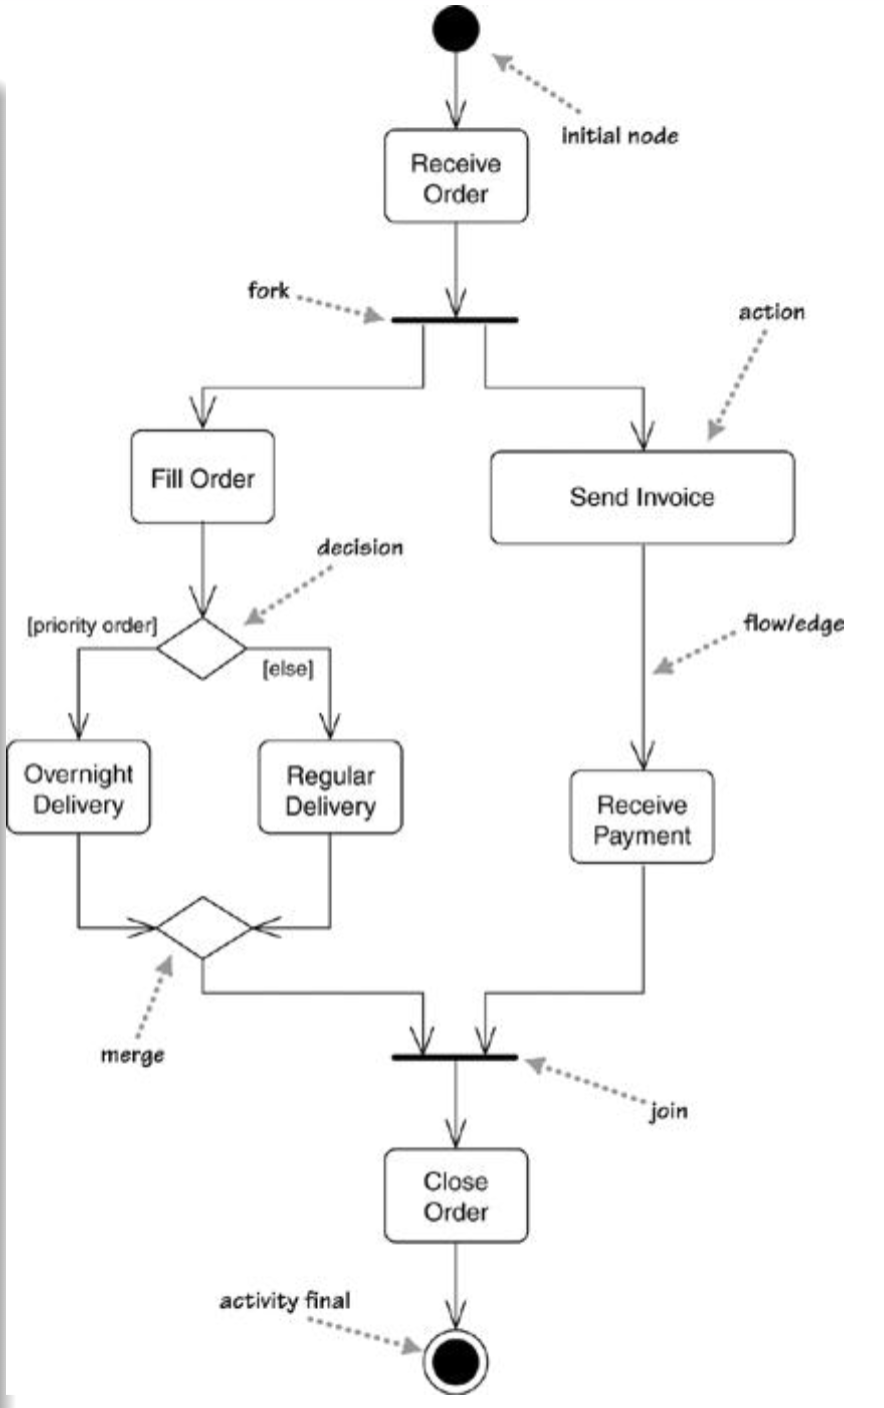
\includegraphics[width=0.4\linewidth]{assets/UML/activity/activity-1.png}}
    \hfill
    \subfloat[Esempio di partizione]{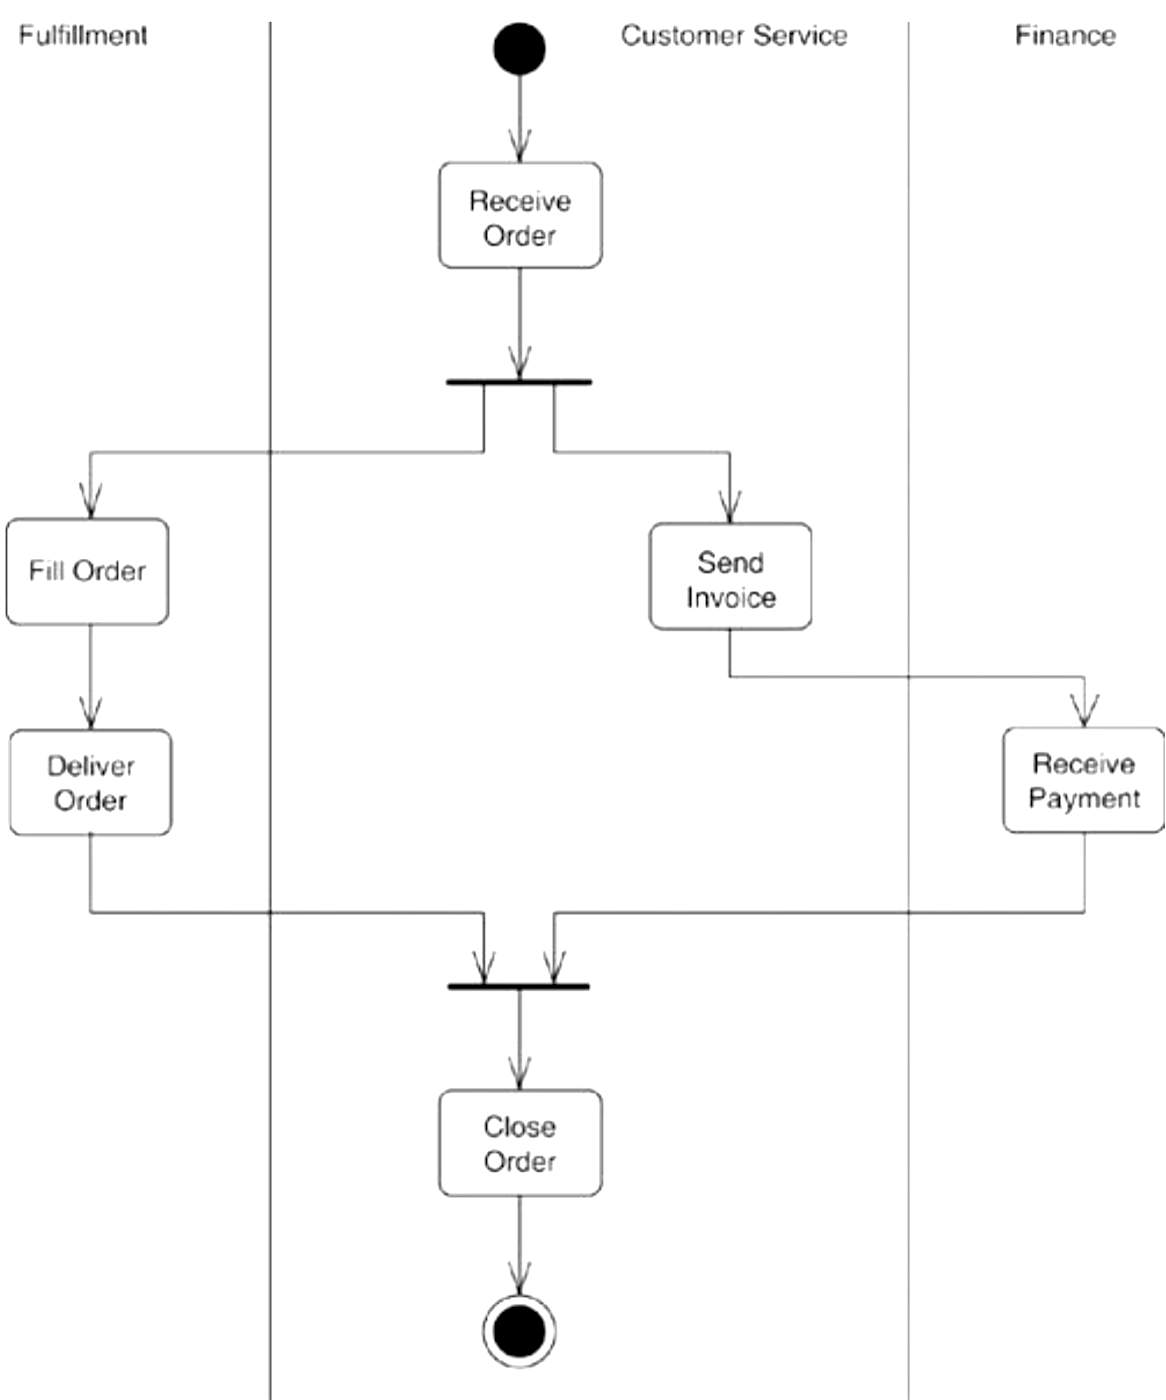
\includegraphics[width=0.55\linewidth]{assets/UML/activity/activity-3.png}}
\end{figure}

\paragraph{Specifiche di Join} Le operazioni di join operano la “sincronizzazione” tra flussi. È possibile introdurre una condizione booleana per la quale si può proseguire (viene rispettata) solo se tutti i flussi paralleli hanno terminato la loro esecuzione.

\paragraph{Partizioni} L'activity diagram può essere partizionato sulla base delle \textit{tipologie di attività} o dell'\textit{entità} adibita a svolgerle. Sono rappresentate tramite un'icona a \textit{rastrello}. Una determinata azione può essere implementata da un metodo; in tal caso si usa la sintassi “nomeClasse::nomeMetodo”. In un diagramma partizionato sono presenti delle \textbf{swim lane}: linee verticali che consentono di separare le competenze.

\begin{figure}[H]
    \subfloat[Diagramma secondario]{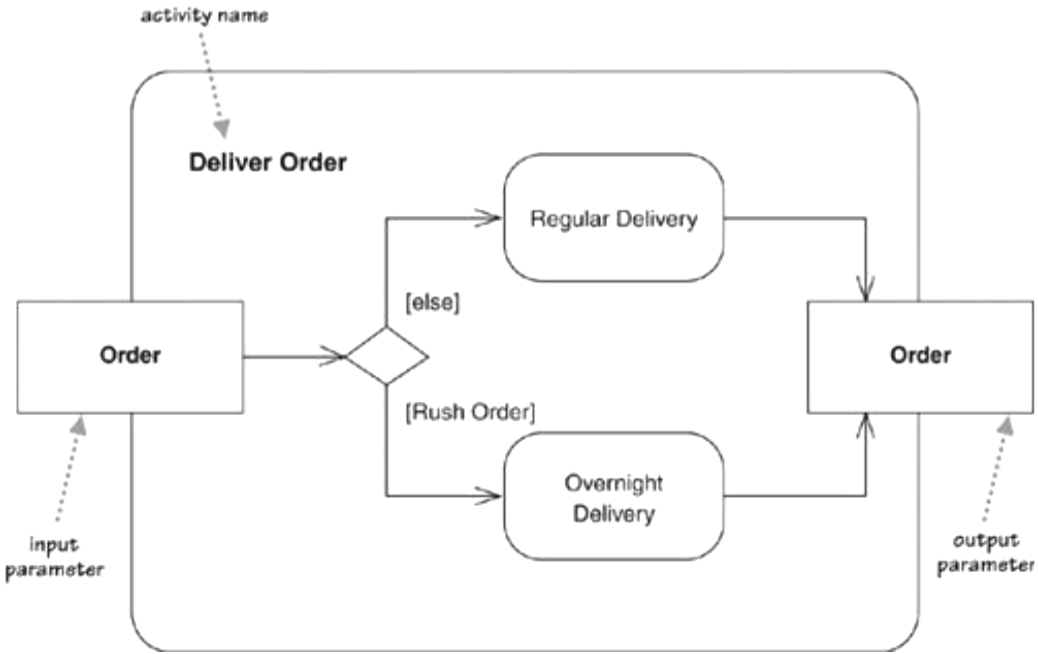
\includegraphics[width=0.55\linewidth]{assets/UML/activity/activity-2.png}}
    \hfill
    \subfloat[Utilizzo di flussi e connettori]{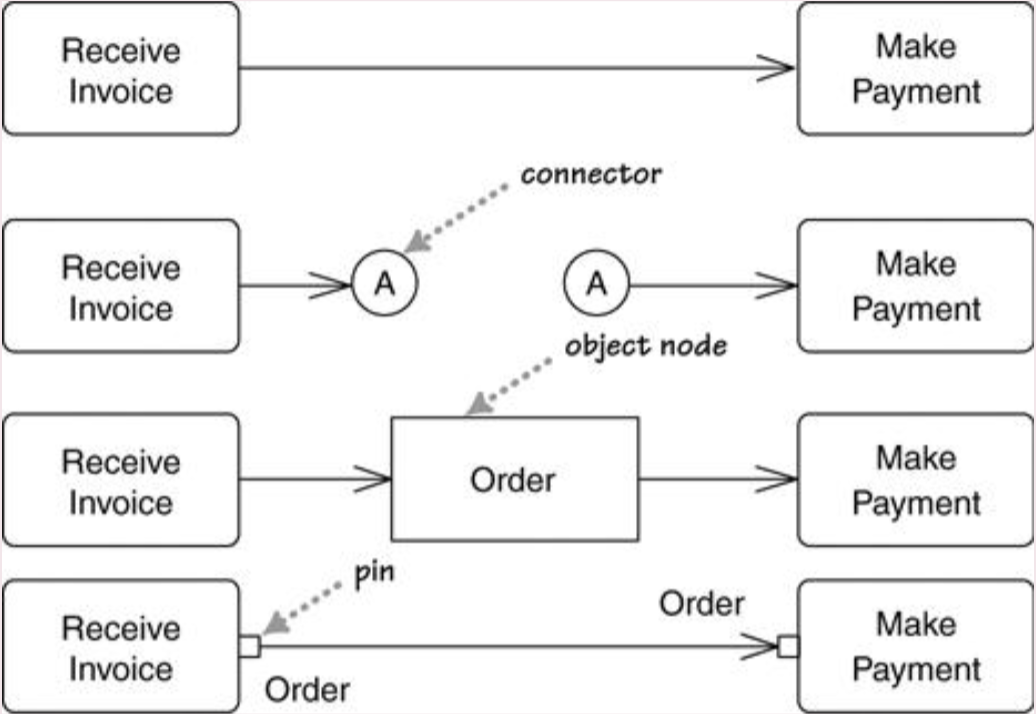
\includegraphics[width=0.4\linewidth]{assets/UML/activity/activity-4.png}}
\end{figure}

\newpage
\paragraph{Segnali} Eventi che il sistema può ricevere o generare da/verso l'esterno. Possono essere \textbf{temporali} (clessidre) o \textbf{personali} (generati da azioni, ad esempio).

\begin{figure}[H]
    \subfloat{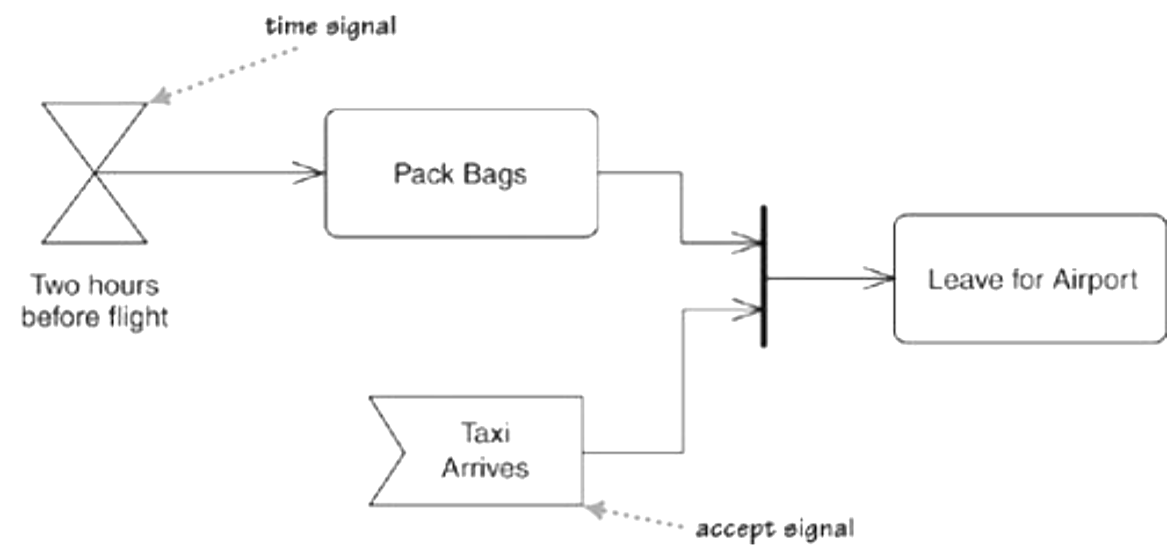
\includegraphics[width=0.455\linewidth]{assets/UML/activity/activity-6.png}}
    \hfill
    \subfloat{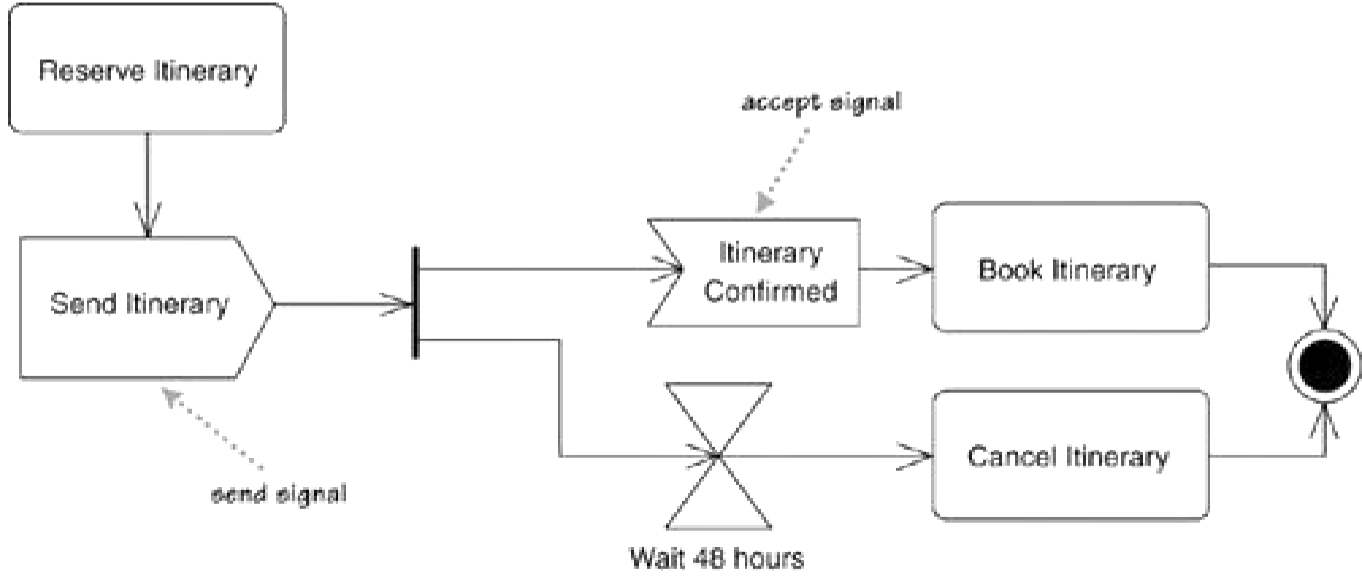
\includegraphics[width=0.5\linewidth]{assets/UML/activity/activity-5.png}}
    \caption{Esempi di utilizzo di \textbf{segnali}}
\end{figure}

\begin{figure}[H]
    \centering
    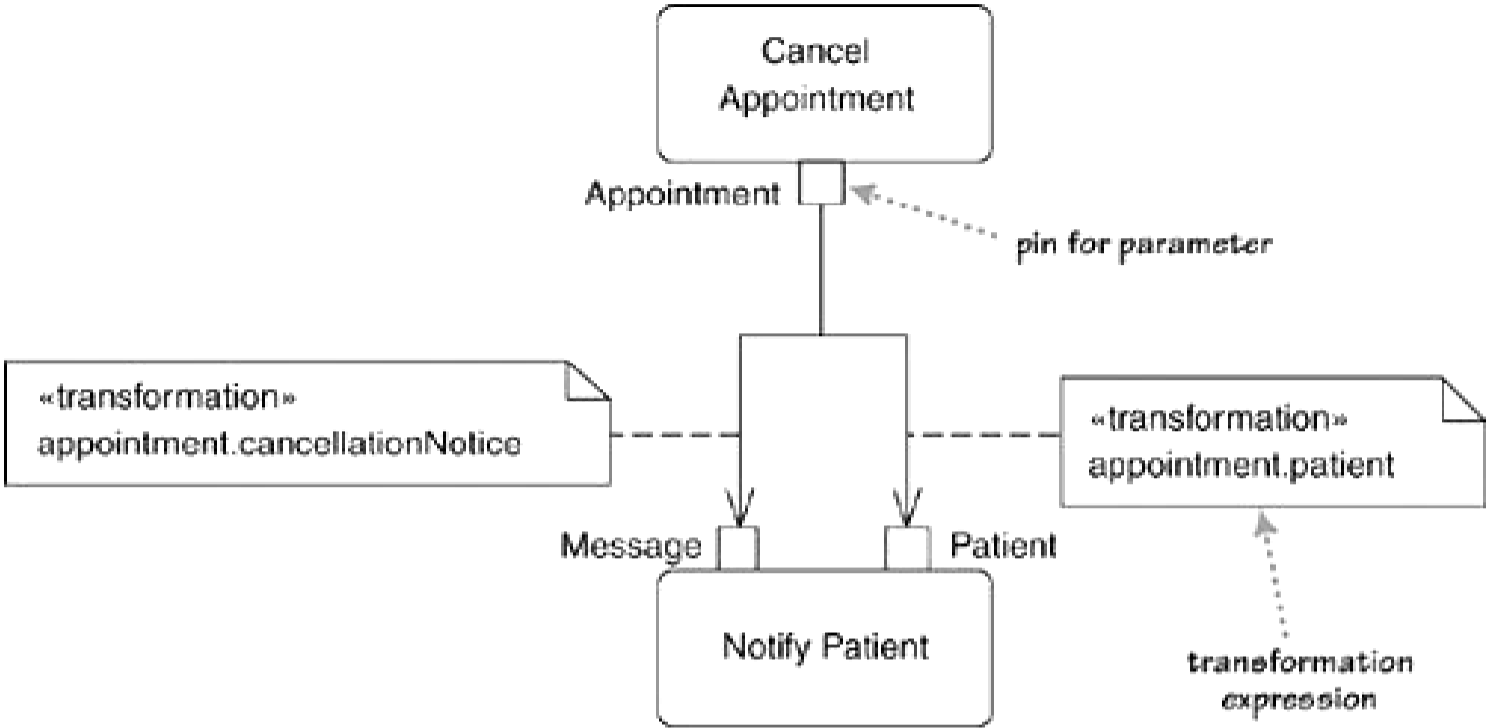
\includegraphics[width=0.75\linewidth]{assets/UML/activity/activity-7.png}
    \caption{I \textbf{pin} consentono di identificare oggetti in input/output per le attività. Le \textbf{trasformazioni} mostrano le modifiche subite dagli oggetti nelle attività.}
\end{figure}

\paragraph{Regione di espansione} Insieme di attività che devono essere eseguite per ogni elemento di una lista di oggetti in ingresso. Restituiscono in output un'altra lista di oggetti.

\begin{figure}[H]
    \centering
    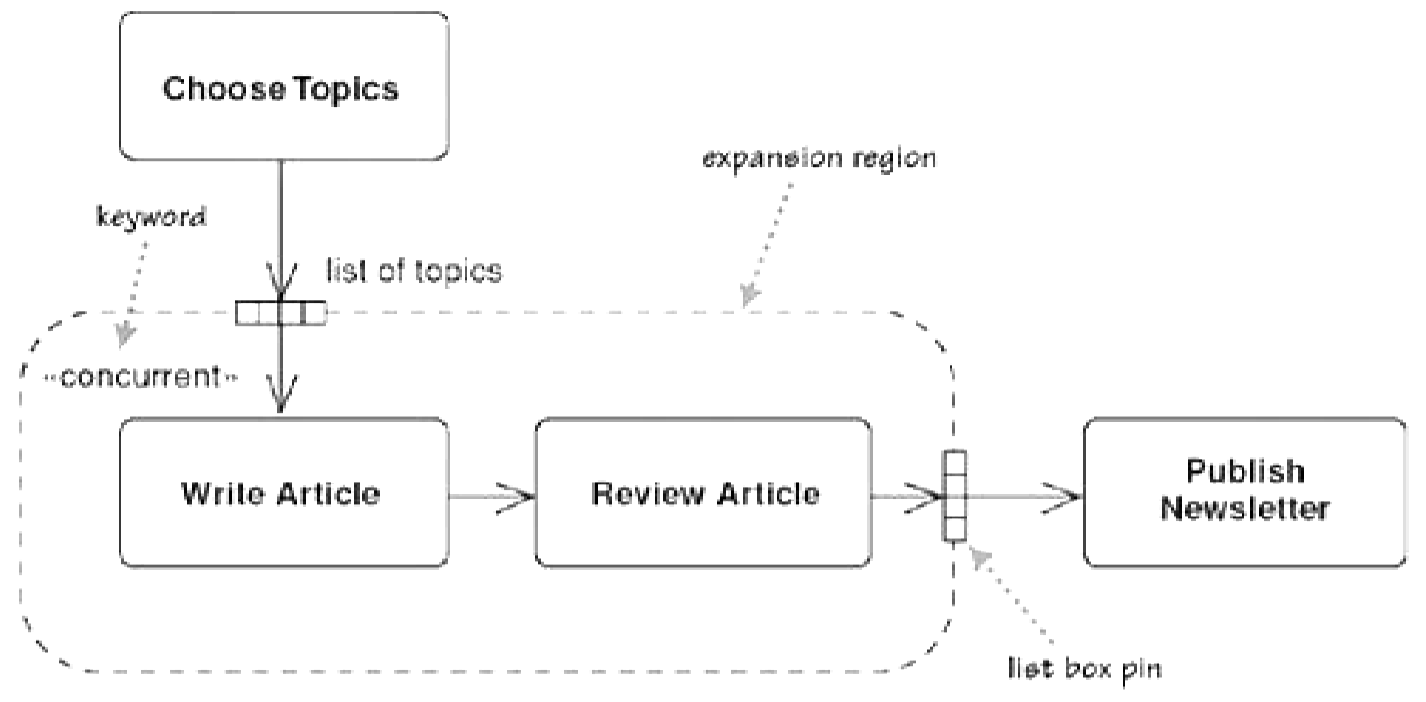
\includegraphics[width=0.8\linewidth]{assets/UML/activity/activity-8.png}
    \caption{Esempio di utilizzo di \textbf{regioni di espansione}}
\end{figure}

\begin{figure}[H]
    \centering
    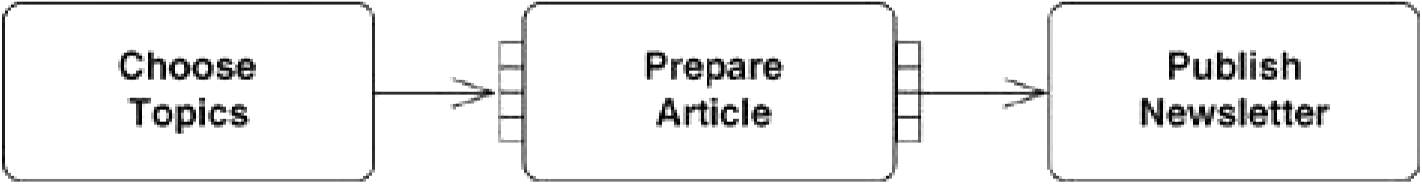
\includegraphics[width=0.8\linewidth]{assets/UML/activity/activity-9.png}
    \caption{Diagramma semplificato risultante a seguito della specifica della regione di espansione}
\end{figure}

\newpage
\subsection{Class}

I \textbf{class diagram} sono i diagrammi UML più utilizzati. Descrivono le \textit{tipologie di oggetti} (classi) che fanno parte del sistema, e le loro relazioni statiche. Nella \textit{prospettiva concettuale} definiscono un vocabolario del dominio applicativo.

\begin{figure}[H]
    \centering
    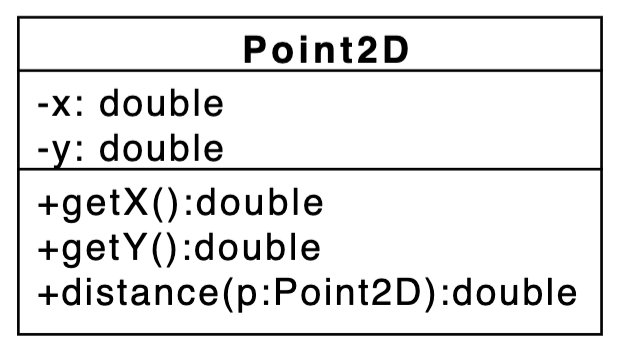
\includegraphics[width=0.5\linewidth]{assets/UML/class/class-1.png}
    \caption{Esempio di definizione di classe}
\end{figure}

\paragraph{Classe} Rappresentata graficamente da rettangoli contenenti almeno il nome della classe e al più le sue caratteristiche. Le caratteristiche (o \textit{feature}) sono divise in \textit{proprietà} e \textit{operazioni}, queste possono avere diversi livelli di visibilità: \textit{public} (+), \textit{private} (-), \textit{protected} (\#) o \textit{package} ($\sim$).

\newpage
\paragraph{Proprietà} Rappresentano le caratteristiche strutturali di una classe (non temporanee, es. parametri in input di un metodo). Si possono esprimere sotto forma di \textit{attributo}:
\begin{center}
    $\langle$visibilità$\rangle$ $\langle$nome$\rangle$ : $\langle$tipo$\rangle$ $\langle$molteplicità$\rangle$ = $\langle$default$\rangle$ \{$\langle$proprietà$\rangle$\}
\end{center}
Dove:
\begin{itemize}
    \item La \textbf{visibilità} è indicata con un simbolo;
    \item Il \textbf{tipo} indica l'insieme di valori assumibili;
    \item La \textbf{molteplicità} vincola il numero di oggetti che possono costituire l'attributo. Espressa come intervallo $[m, n]$;
    \item Il \textbf{default} è valore predefinito;
    \item La \textit{proprietà} è una stringa che indica vincoli aggiuntivi (es. \textit{read-only} o \textit{frozen}). Per specificare il criterio di l'ordinamento si usano \textit{ordered} o \textit{sorted}
\end{itemize}
Si esprimono \textit{attributi} (il cui tipo è non significativo) e \textit{associazioni} (il cui tipo è significativo, espresso da un'altra classe del sistema).
Non esiste un metodo univoco di traduzione, ma in linguaggi moderni quali Java le proprietà corrispondono ai campi (spesso esposti tramite metodi accessori quali \textit{get} e \textit{set} o \textit{wrapper} per collezioni), mentre le operazioni corrispondono ai metodi.

\subparagraph{Proprietà derivata} È una proprietà per la quale non serve introdurre un campo per memorizzarla e può essere calcolata a partire da altre proprietà, è indicata come attributo accompagnato dal simbolo "$/$" corredato da una nota che esprime come ottenerla. Esprime un vicolo (concetto di \textit{invariante di classe}) per le proprietà coinvolte.

\begin{figure}[H]
    \centering
    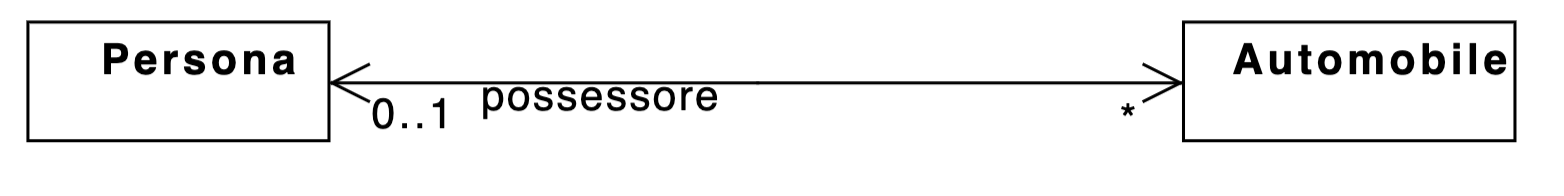
\includegraphics[width=0.75\linewidth]{assets/UML/class/class-3.png}
    \caption{\textbf{Associazione bidirezionale} - ogni oggetto Persona può avere una collezione di oggetti Automobile; ogni oggetto Automobile può avere proprietà opzionale di tipo Persona}
\end{figure}

\newpage
\paragraph{Operazioni} Rappresentano caratteristiche funzionali delle istanze di una classe (azioni invocabili su di esse). Vengono rappresentate tramite stringhe composte come segue:
\begin{center}
        $\langle$visibilità$\rangle$ $\langle$nome$\rangle$(lista\_parametri) : $\langle$tipo\_ritorno$\rangle$ \{$\langle$proprietà$\rangle$\}
\end{center}
La lista dei parametri va specificata. Ogni parametro è separato da virgole ed è espresso come segue:
\begin{center}
        $\langle$direzione$\rangle$ $\langle$nome$\rangle$ : $\langle$tipo$\rangle$ = $\langle$default$\rangle$
\end{center}
Dove:
\begin{itemize}
    \item La \textbf{direzione} indica se il parametro è in input (\textit{in}), in output (\textit{out}) o entrambi (\textit{inout});
    \item La \textbf{proprietà} indica se l'operazione cambia o meno lo stato del sistema. Se non lo cambia si aggiunge la stringa \textit{query}.
\end{itemize}
Nota: Java non permette di specificare la direzione o valore default dei parametri.
UML distingue operazioni (dichiarazione di una procedura) e metodi (corpo dell'operazione).

\subparagraph{Static} Vengono definiti \textit{static} quegli attributi o quelle operazioni che si riferiscono alla classe e non alle sue istanze. Nel diagramma le caratteristiche \textit{static} vengono sottolineate.

\paragraph{Generalizzazione} Anche i class diagram ammettono relazioni di generalizzazione che partono da classi \textit{specializzate} e puntano ad una classe \textit{generale}. In Java viene espressa con il concetto di \textit{ereditarietà} (classe specializzata sottoclasse di classe generica o superclasse - \textbf{Principio di sostituibilità di Liskov}, vedi \ref{liskov}).

\begin{figure}[H]
    \centering
    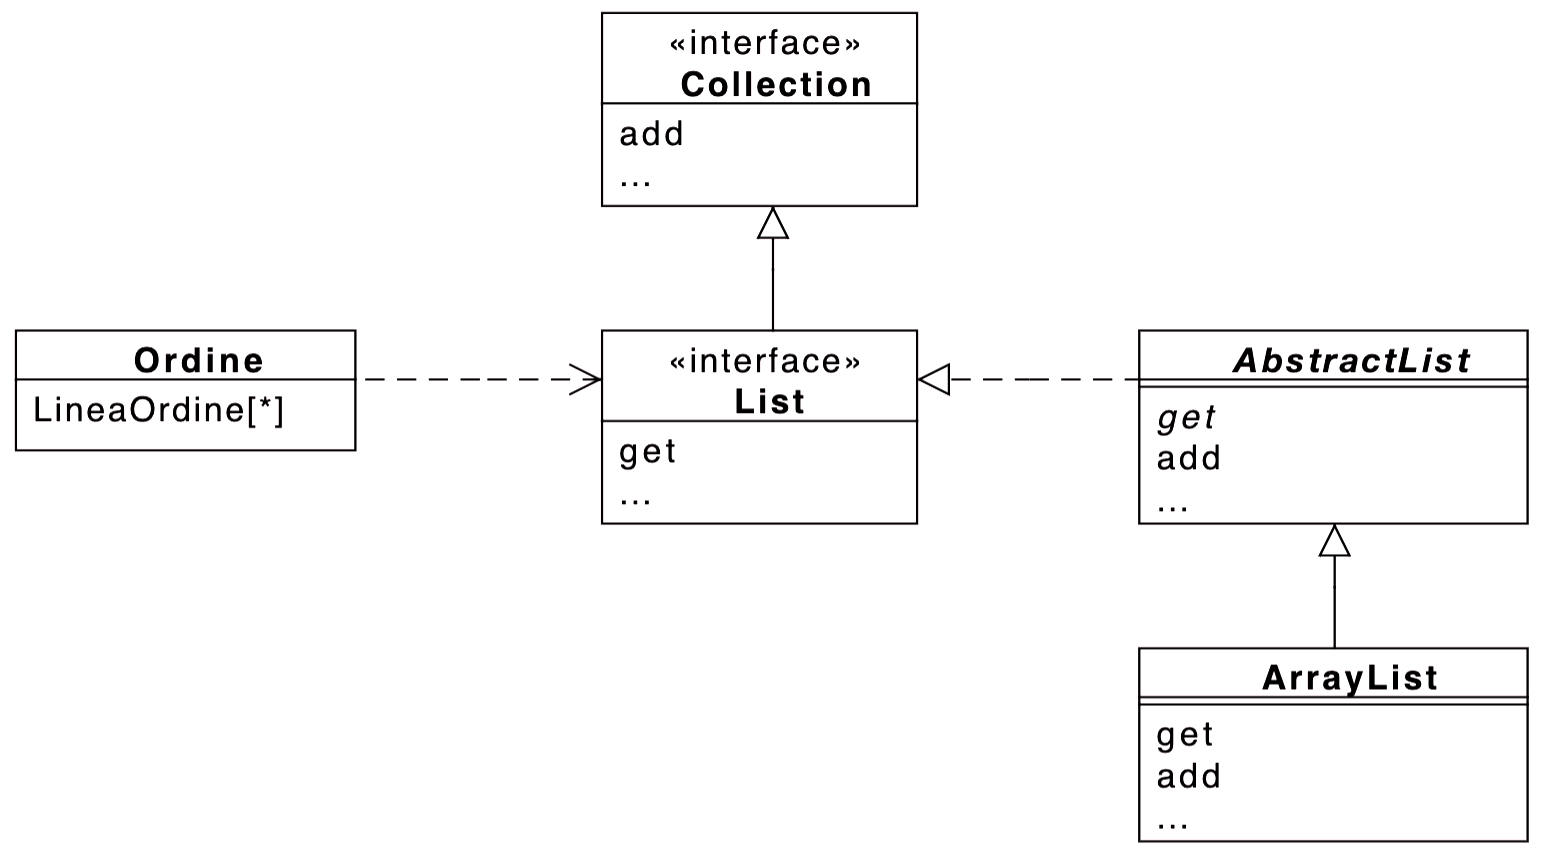
\includegraphics[width=0.75\linewidth]{assets/UML/class/class-8.png}
    \caption{Esempio di generalizzazione}
\end{figure}

\newpage
Di seguito un esempio in Java che non rispetta il principio di Liskov:
\begin{verbatim}
public class Rettangolo {
    private double base;
    private double altezza;

    public void setBase(double b){ base = b;}
    ...
    public double getBase(){return base;}
    ...
    public double getArea(){return base * altezza;}
}

public class Quadrato extends Rettangolo {
    public Quadrato(double l) {
        super(l, l);
    }
    ...
}
\end{verbatim}
Sebbene \textit{geometricamente} un quadrato è un rettangolo, l'implementazione è \textbf{sbagliata} in quanto non deve essere possibile sostituire un Quadrato ad un Rettangolo laddove ci si aspetta il secondo. Si hanno quindi due alternative: rendere le classi \textbf{immutabili} o \textbf{separarle}.

I class diagram ammettono il concetto di \textit{classe astratta} (non istanziabile) e \textit{operazione astratta} (solo dichiarata, priva di corpo), convenzionalmente indicate dal nome scritto in corsivo.

È anche possibile definire delle \textit{interfacce} (insieme di operazioni) indicate dalla parola chiave $\langle\langle$interface$\rangle\rangle$.

La relazione che lega interfaccia e classe (astratta o concreta) si dice \textit{realizzazione} e viene rappresentata da una linea tratteggiata con la punta chiusa e vuota che parte dalla classe e punta all'interfaccia.

\begin{figure}[H]
    \centering
    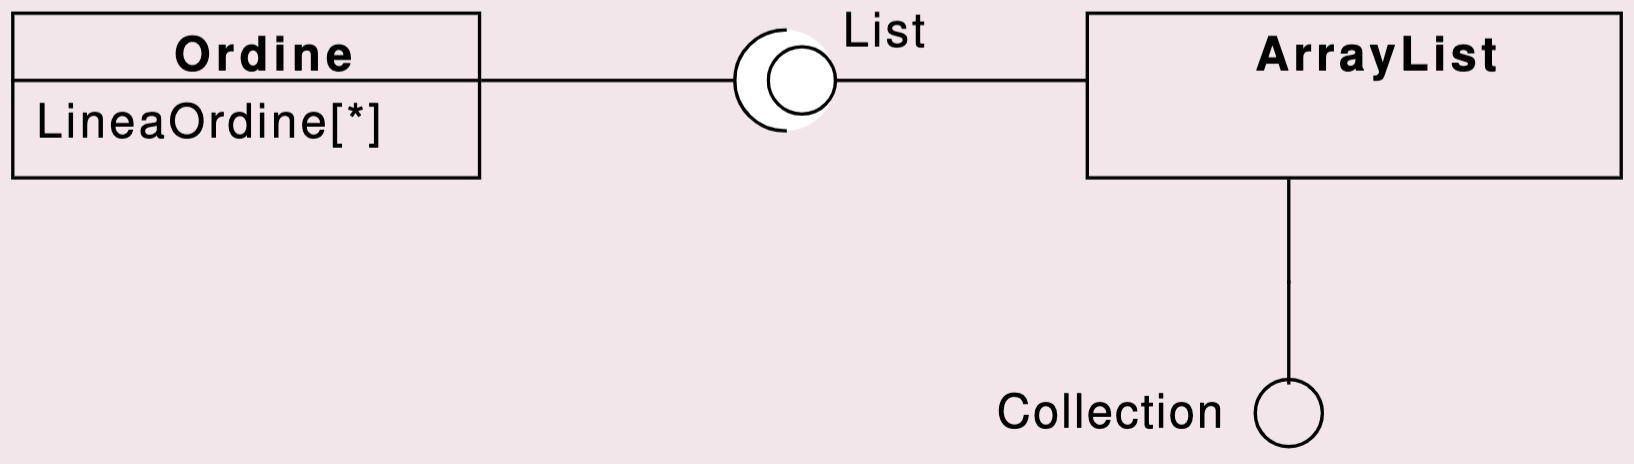
\includegraphics[width=0.75\linewidth]{assets/UML/class/class-9.png}
    \caption{Esempio di utilizzo della notazione \textit{lollipop} (classe fornisce interfaccia) e notazione \textit{socket} (classe richiede interfaccia)}
\end{figure}

\begin{figure}[H]
    \centering
    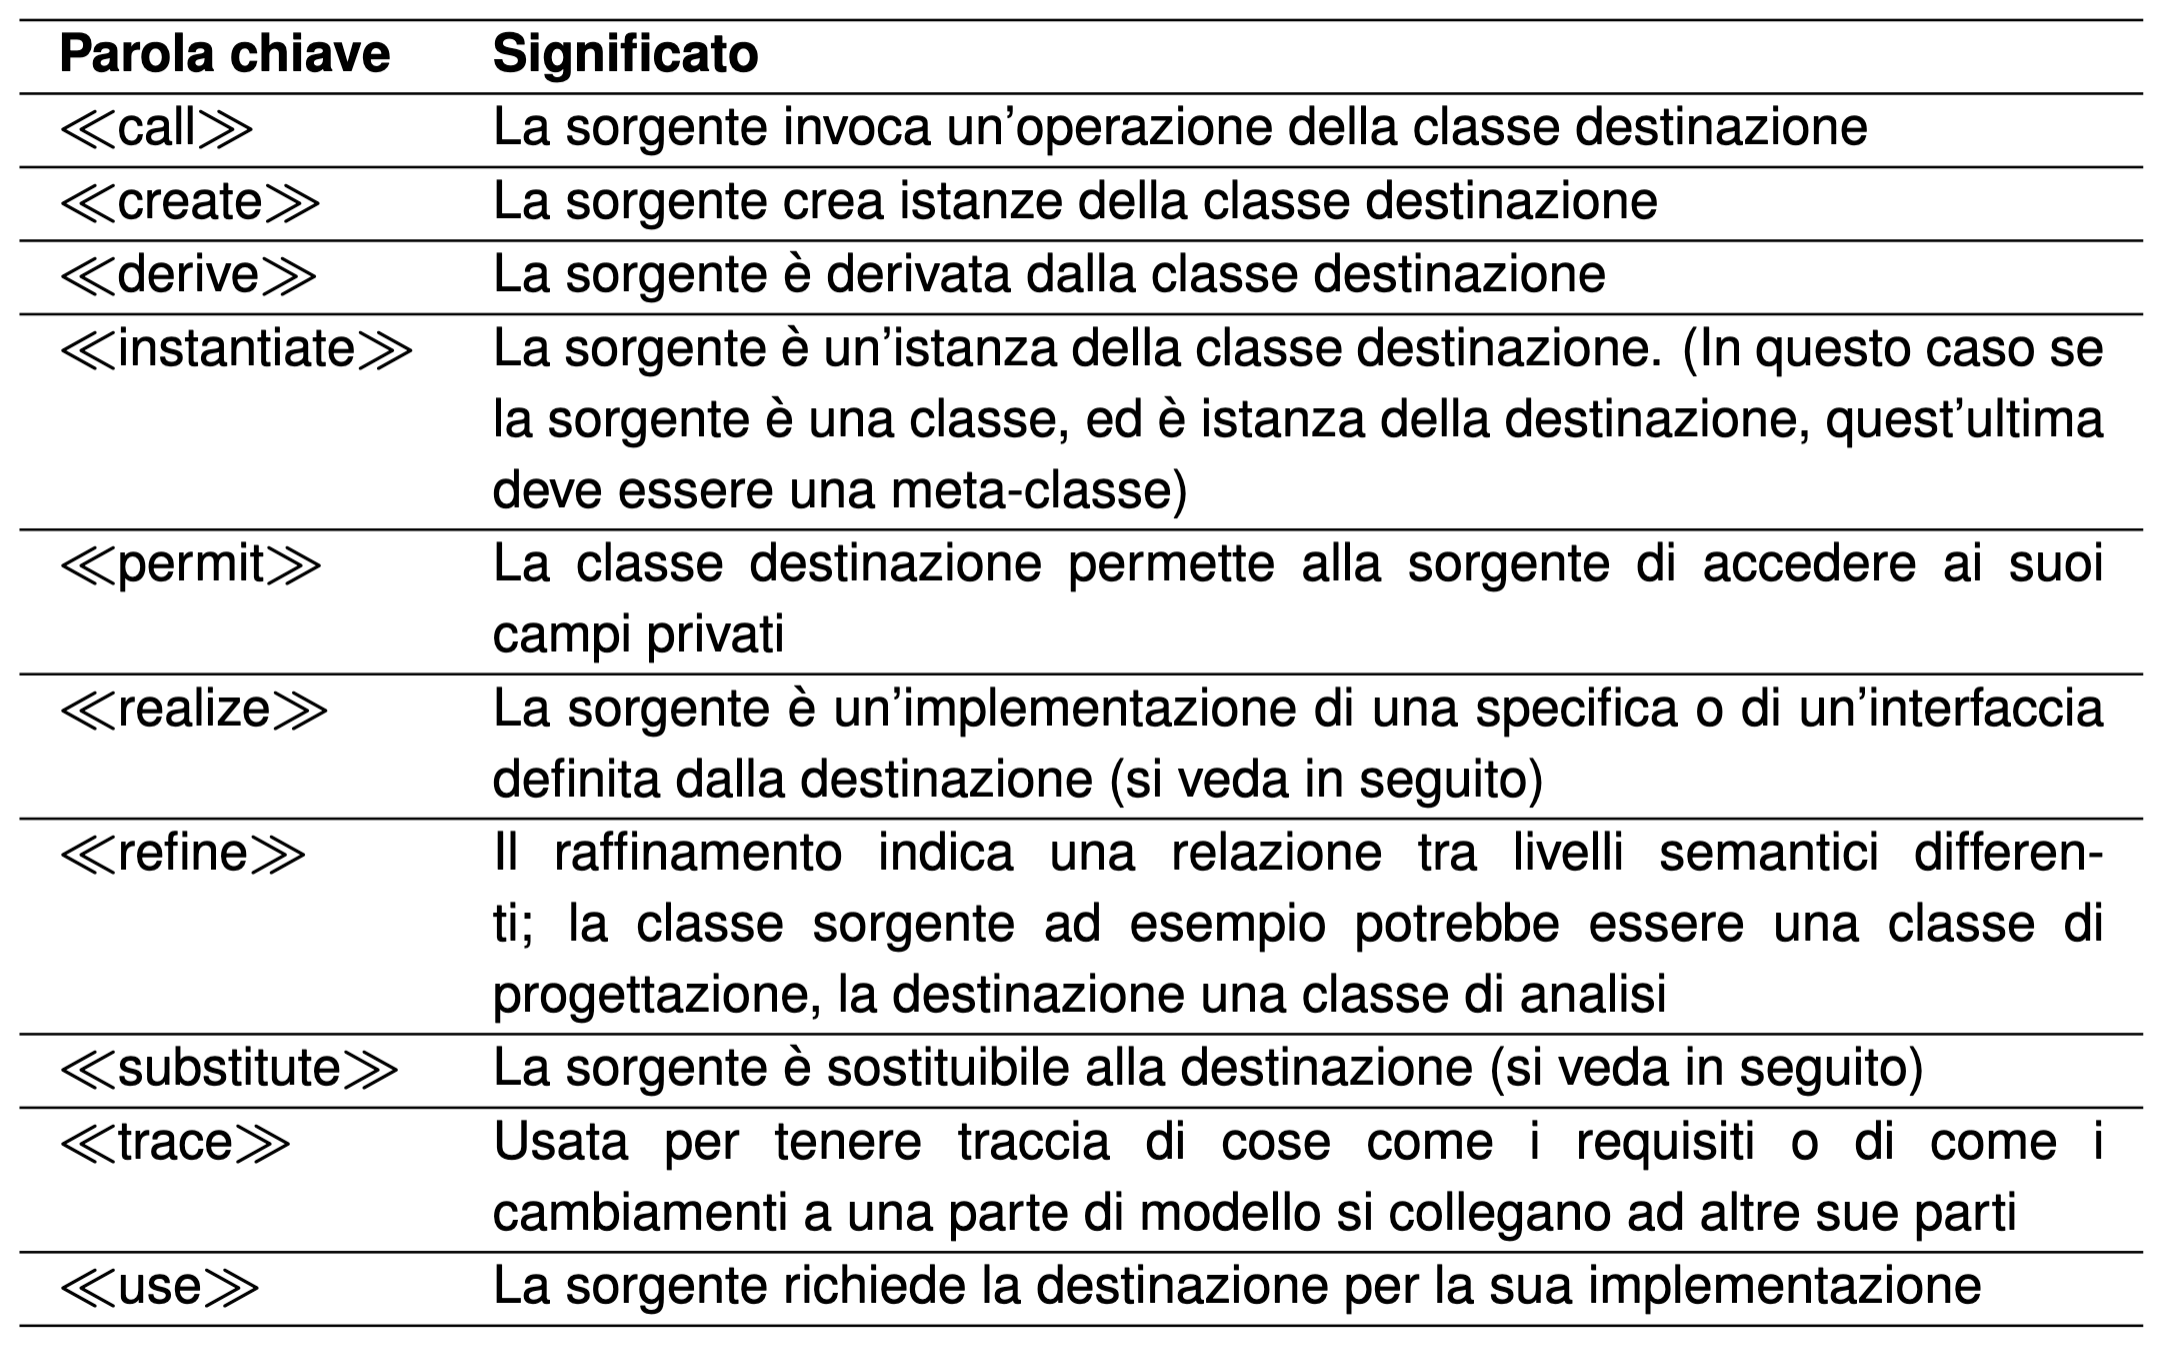
\includegraphics[width=1\linewidth]{assets/UML/class/class-10.png}
    \caption{I class diagram prevedono \textbf{dipendenze}, relazioni unidirezionali tra una classe \textit{client} (da cui parte la freccia) ad una classe \textit{supplier} (in cui punta la freccia). Una qualsiasi modifica alla classe supplier ha effetto sulla classe client (non viceversa), in più NON gode di proprietà transitiva. È inoltre possibile definire dipendenze \textit{custom} (personalizzate)}.
\end{figure}

\begin{figure}[H]
    \centering
    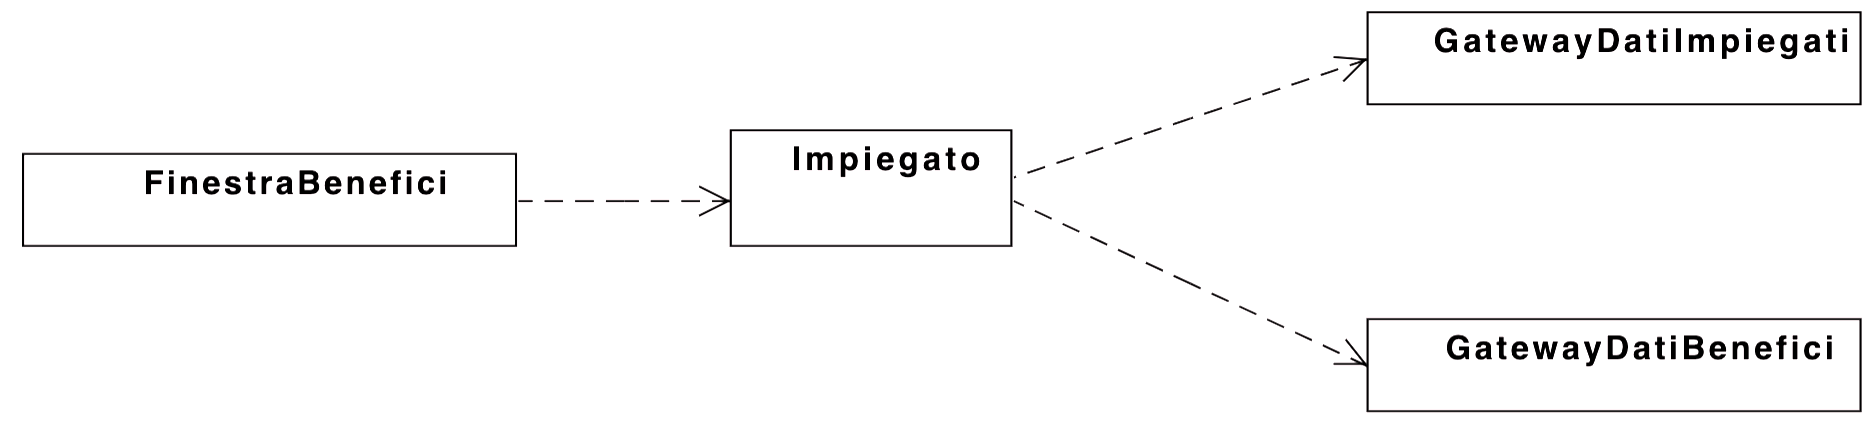
\includegraphics[width=1\linewidth]{assets/UML/class/class-5.png}
    \caption{Esempio di utilizzo del concetto di dipendenza}
\end{figure}

I class diagram consentono l'uso di interfacce e classi \textbf{parametriche}: nel codice, i campi e i parametri/risultati dei metodi sono di tipo generico (sussiste a tempo di compilazione, es. Java) o \textit{template} (sussiste a runtime, es C++).

\begin{figure}[H]
    \centering
    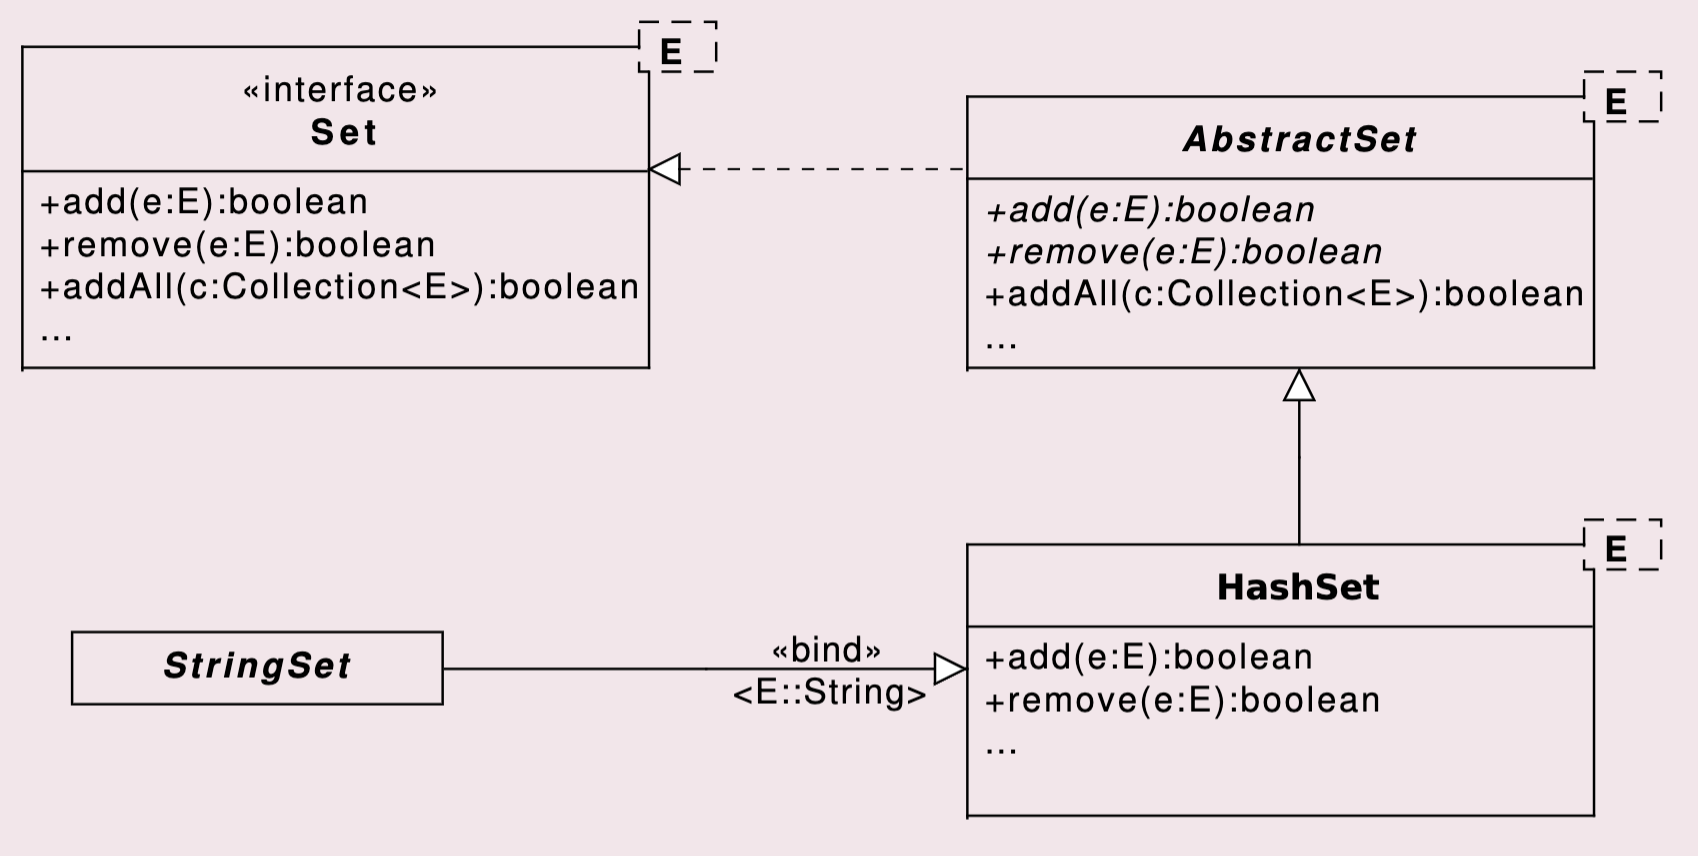
\includegraphics[width=1\linewidth]{assets/UML/class/class-11.png}
    \caption{Esempio di \textbf{derivazione}: classe discendente da una classe parametrica che sostituisce il tipo generico con uno concreto tramite \textit{bind}}
    
\end{figure}
L'introduzione di una classe tramite derivazione fa si che si abbia una relazione di \textit{raffinamento}. 

I tipi che possono assumere solo un set finito di valori prefissati sono modellati tramite \textit{enumerazioni}. 

Una classe \textit{attiva} è una classe che esegue e controlla autonomamente il proprio thread (es. la classe Thread di Java).

\paragraph{Aggregazione} È una forma di associazione in cui l'oggetto destinazione è un \textit{componente} della classe sorgente, il quale viene \textit{aggregato}.

\begin{figure}[H]
    \centering
    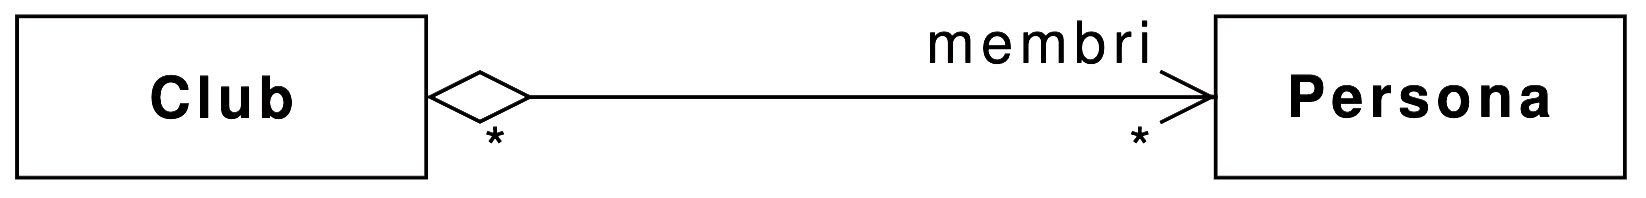
\includegraphics[width=1\linewidth]{assets/UML/class/class-6.png}
    \caption{Esempio di aggregazione}
\end{figure}

\paragraph{Composizione} È una forma di aggregazione in cui l'oggetto sorgente è composto da un insieme di oggetti del tipo destinazione.

\begin{figure}[H]
    \centering
    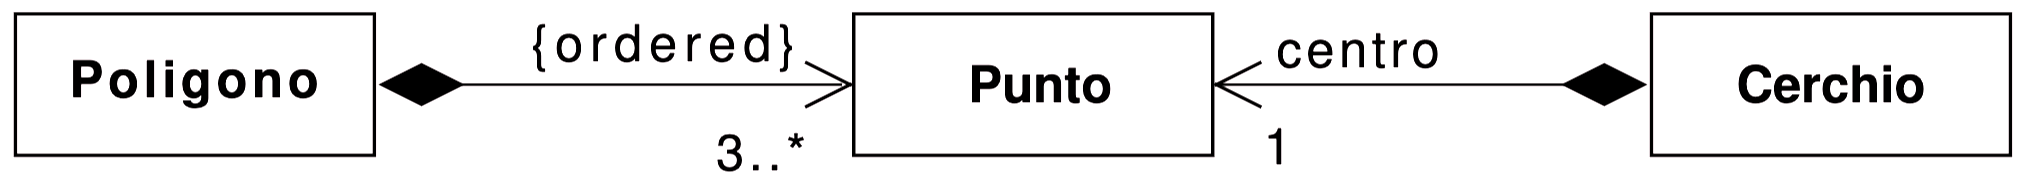
\includegraphics[width=1\linewidth]{assets/UML/class/class-7.png}
    \caption{Esempio di composizione}
\end{figure}
Le differenze tra composizione e aggregazione sono le seguenti:
\begin{itemize}
    \item La \textit{composizione} è una relazione esclusiva: l'oggetto componente può far parte di un solo oggetto composto (uno ad uno); nell'\textit{aggregazione} può esistere una relazione uno a molti.
    \item Nella \textit{composizione}, l'istanza composta è responsabile dell'esistenza (creazione, modifica e cancellazione) delle istanze componenti, se viene distrutta anche i suoi componenti vengono distrutti; nell'\textit{aggregazione} l'oggetto componente esiste in maniera indipendente dall'aggregato.
\end{itemize}

\begin{figure}[H]
    \centering
    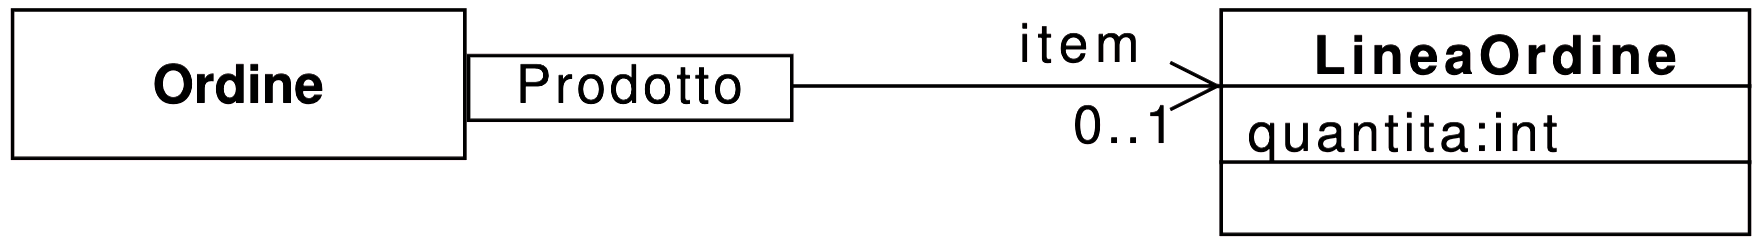
\includegraphics[width=1\linewidth]{assets/UML/class/class-12.png}
    \caption{Esempio di \textbf{associazione qualificata} in cui l'oggetto Ordine possiede più oggetti di tipo LineaOrdine, ma al più uno per ogni oggetto Prodotto (detto \textit{qualificatore}, una sorta di chiave). Implementata tramite array associativi quali mappe, tabelle hash, dizionari, ecc...}
\end{figure}

\vspace{20pt}

\begin{figure}[H]
    \centering
    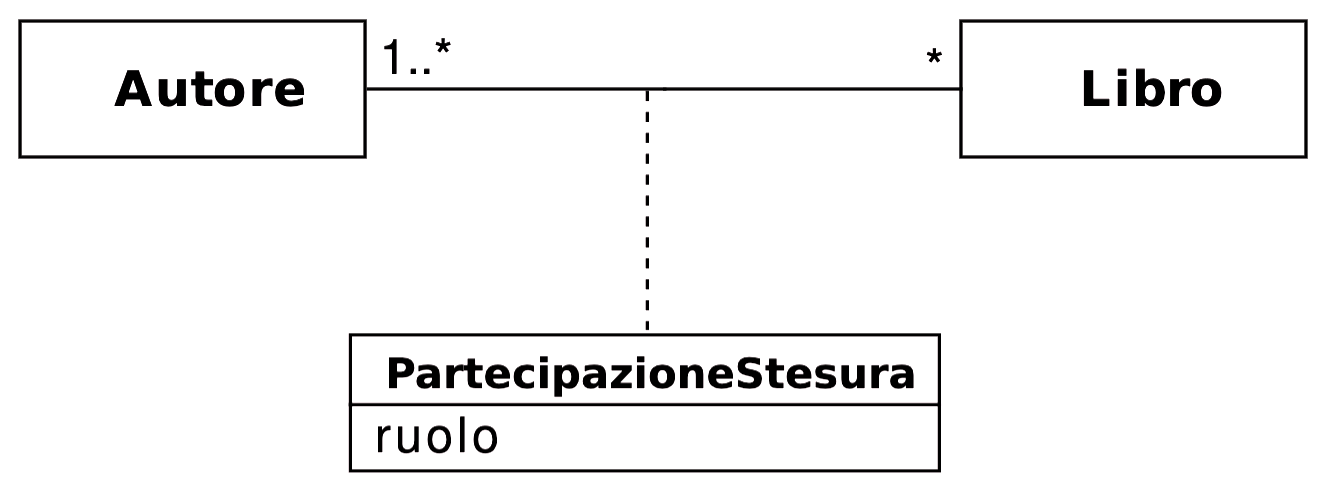
\includegraphics[width=1\linewidth]{assets/UML/class/class-13.png}
    \caption{Esempio di \textbf{classe associativa}: garantisce che per ogni coppia di oggetti associati esista una sola istanza della classe associativa.}
\end{figure}

\vspace{20pt}

\begin{figure}[H]
    \centering
    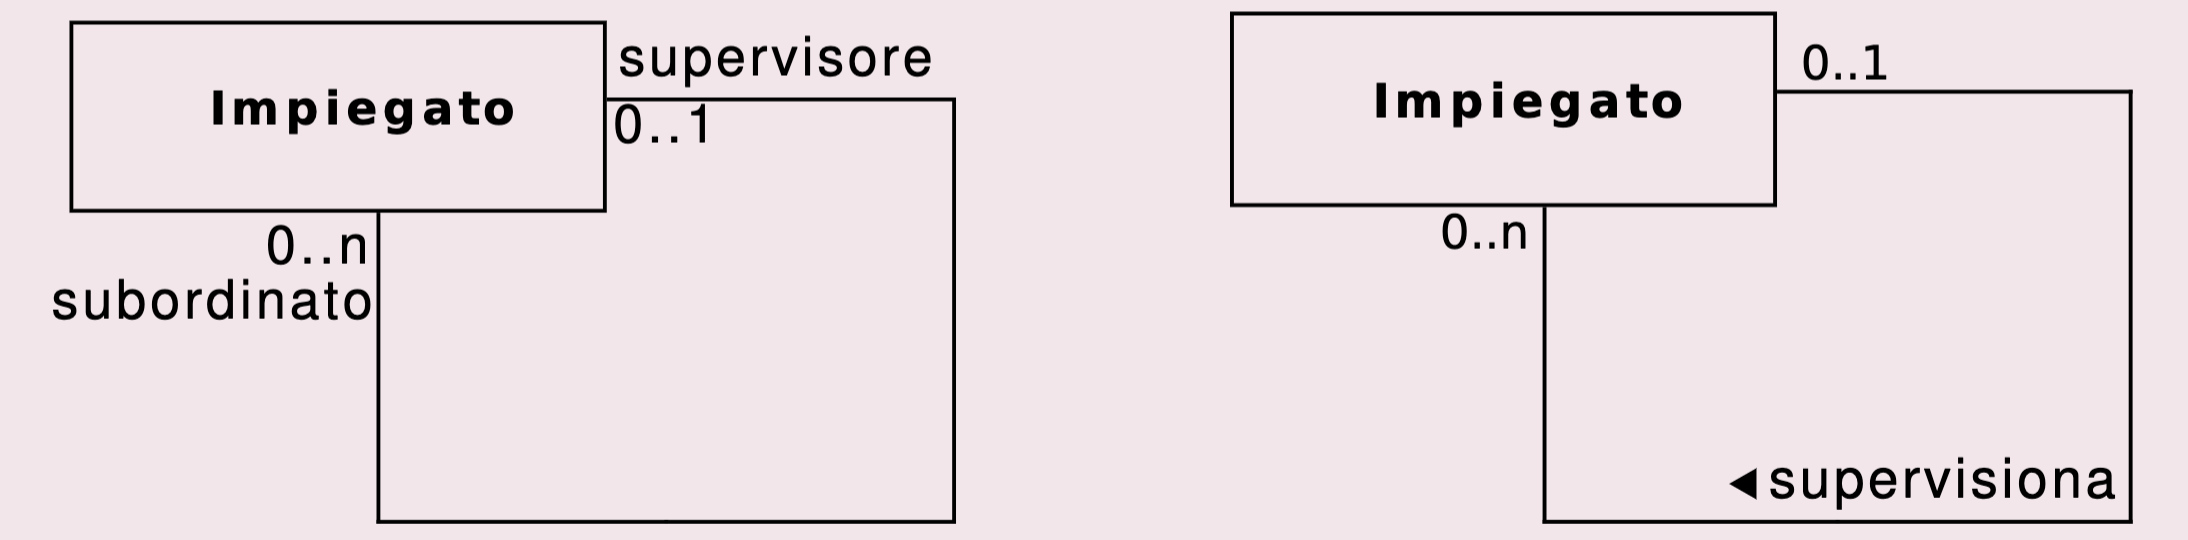
\includegraphics[width=1\linewidth]{assets/UML/class/class-14.png}
    \caption{Esempio di \textbf{associazione riflessiva}: classe sorgente e classe destinazione coincidono, ogni istanza della classe possiede proprietà del suo stesso tipo}
\end{figure}

\vspace{20pt}

\begin{figure}[H]
    \centering
    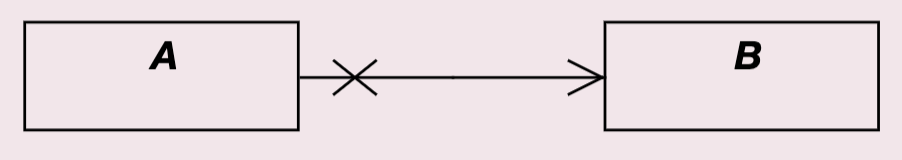
\includegraphics[width=1\linewidth]{assets/UML/class/class-15.png}
    \caption{Concetto di \textbf{non navigabilità}}
\end{figure}

\newpage
\subsection{Communication}

I \textbf{communication diagram}, in maniera simile agli \textit{state diagram}, mostrano il funzionamento collettivo di un gruppo di partecipanti. L'enfasi è posta sui \textbf{messaggi scambiati} (non sul ciclo di vita) e sulle attività svolte da ciascun partecipante.

\paragraph{Partecipante} È un'\textbf{entità del dominio applicativo} nella \textit{prospettiva concettuale}, un \textbf{oggetto} nella \textit{prospettiva software}. Rappresentato da box con angoli smussati. I box sono collegati da linee continue, le quali possono:
\begin{itemize}
    \item tradurre associazioni statiche (tra partecipanti, \textit{compile-time})
    \item introdurre associazioni dinamiche (tra partecipanti, nascono e muoiono a \textit{run-time})
\end{itemize}

\paragraph{Messaggio} Rappresentato da frecce etichettate con l'azione corrispondente e numerato in maniera nidificata. Si usa:
\begin{itemize}
    \item $\langle\langle$create$\rangle\rangle$ per la creazione di partecipanti
    \item $\langle\langle$delete$\rangle\rangle$ per la distruzione di partecipanti
\end{itemize}
Inoltre, è possibile inserire lettere nelle etichette per indicare il thread che esegue l'operazione.

\begin{figure}[H]
    \centering
    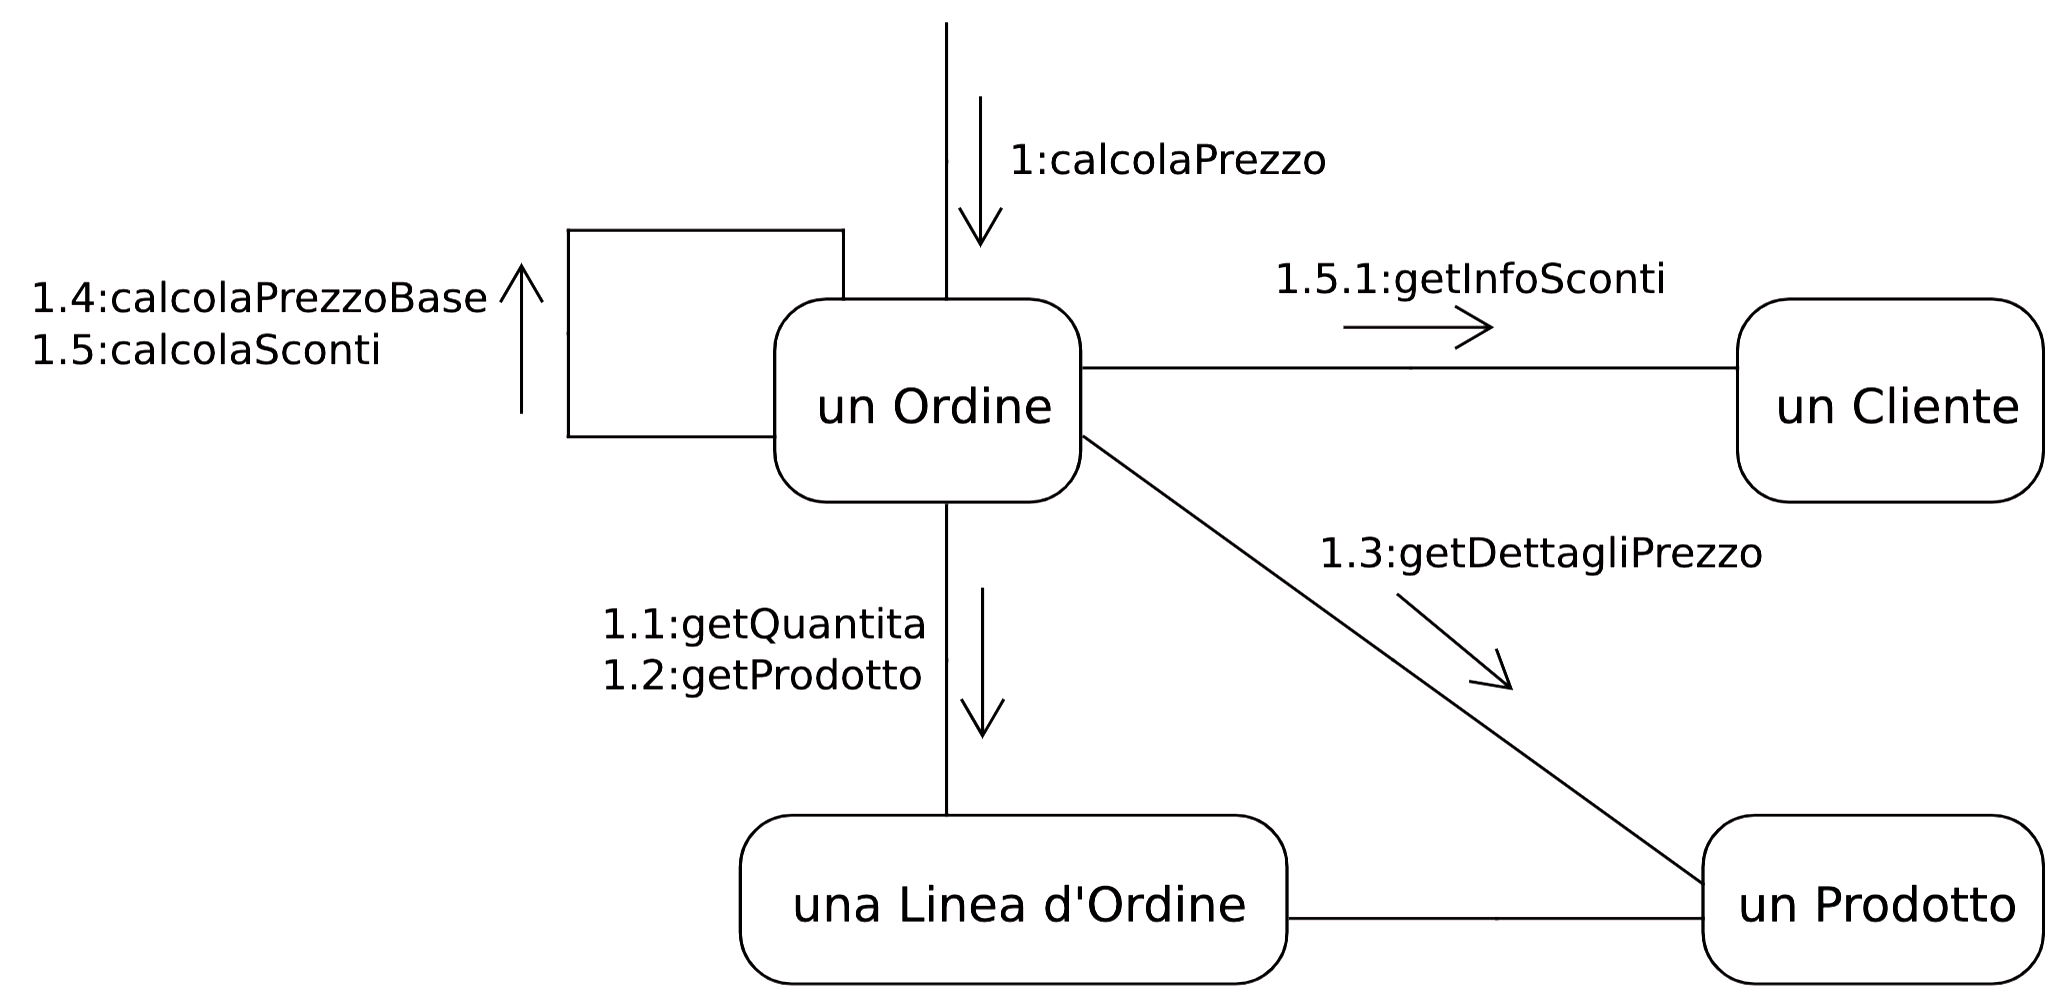
\includegraphics[width=0.75\linewidth]{assets/UML/communication/communication-1.png}
    \caption{Esempio di communication diagram a \textit{controllo centralizzato}.}
\end{figure}

\newpage
\subsection{Componenti}

Uno degli argomenti più dibattuti nella POO è la differenza tra i concetti di \textit{classe} e \textit{componente}. Si può dire che un \textit{componente} è un'entità dotata di interfaccia standard, potenzialmente sostituibile da un altro componente dotato di interfaccia simile (che offre le stesse funzionalità). Un componente può coincidere con: una classe, una porzione di essa o un insieme di classi.

\begin{figure}[H]
    \centering
    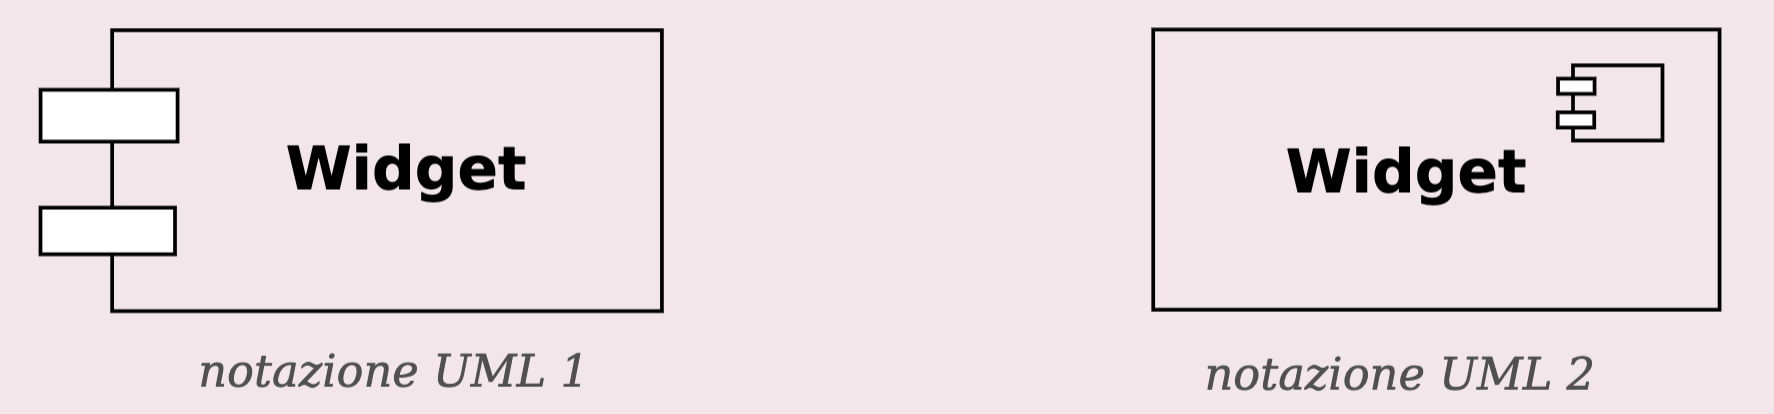
\includegraphics[width=0.75\linewidth]{assets/UML/component/component-1.png}
    \caption{Notazione del componente nelle versioni UML. Un componente complesso può essere rappresentato come struttura composita.}
\end{figure}

\paragraph{Nota} I collegamenti tra componenti sono basati sulle interfacce fornite e richieste.

\begin{figure}[H]
    \centering
    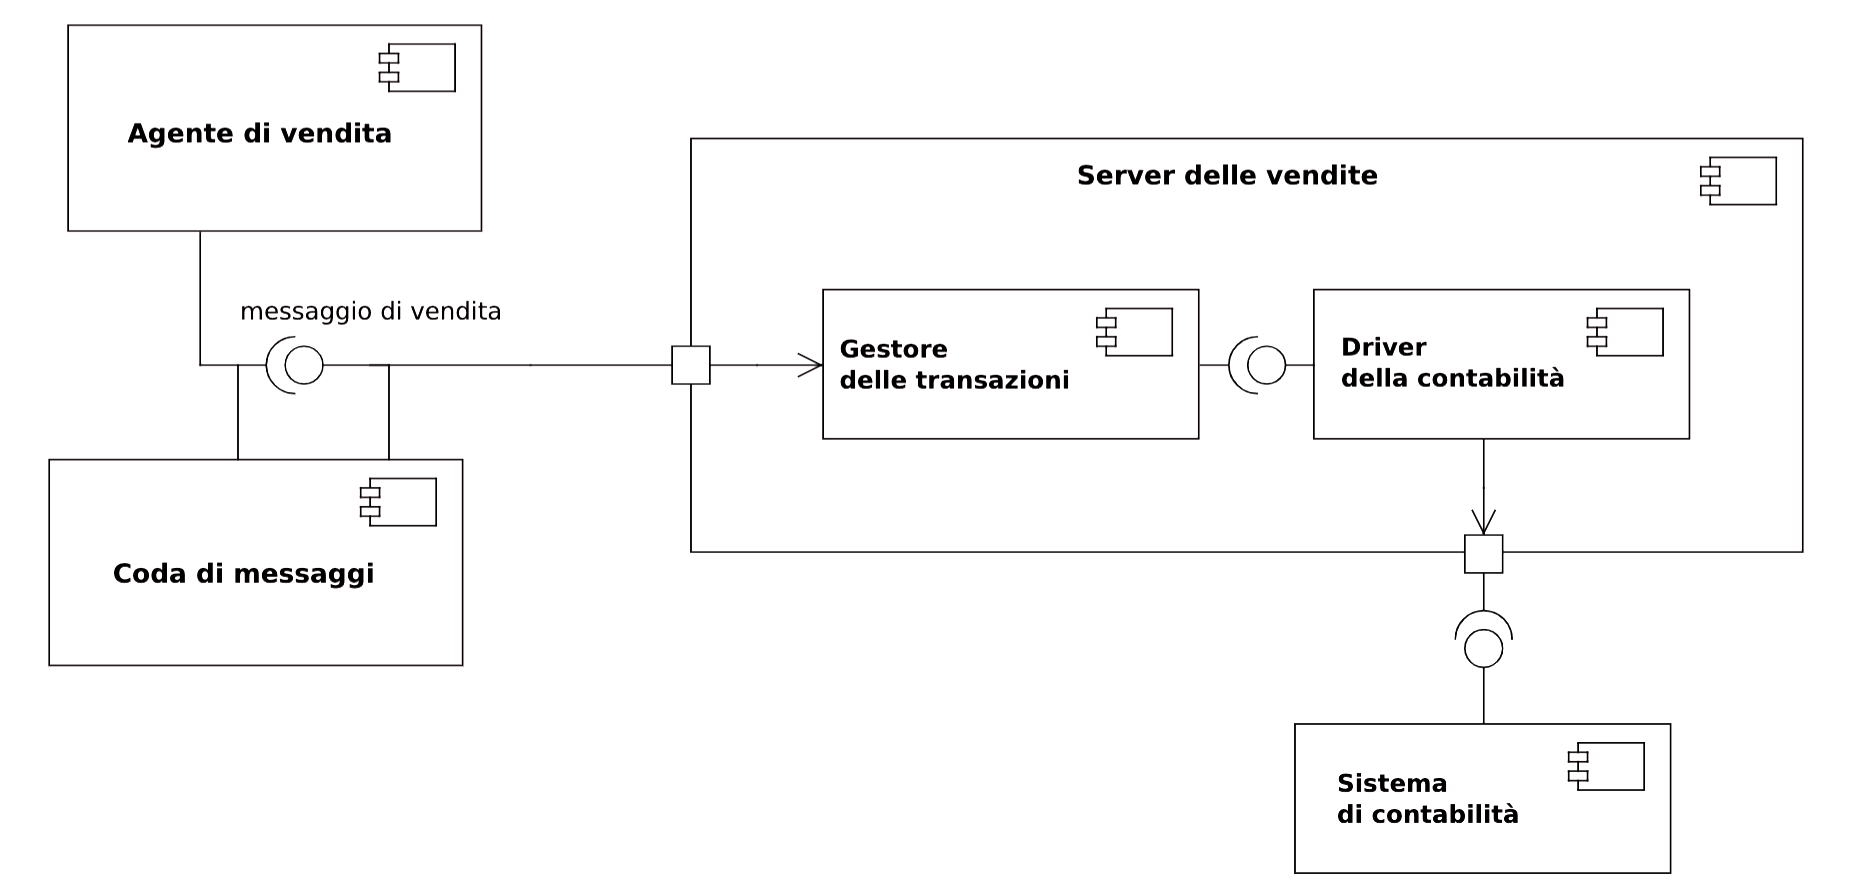
\includegraphics[width=0.75\linewidth]{assets/UML/component/component-2.png}
    \caption{Esempio di component diagram. L'agente di vendita comunica con il server se la rete è disponibile, con la coda altrimenti.}
\end{figure}

\newpage
\subsection{Deployment}

I \textbf{deployment diagram} rappresentano la disposizione fisica dei componenti del sistema software nel contesto applicativo. Il loro modello è rappresentato come un insieme di \textit{nodi}.

\paragraph{Nodo} Contiene uno o più elaborati (\textit{artifact}): manifestazioni fisiche del sistema software (eseguibili, script di configurazione, librerie, jar, file di dati, documenti HTML, ecc...)

I nodi sono collegati da linee continue dette \textit{path} che forniscono informazioni sulla comunicazione tra essi (es. canale usato, protocollo adottato). I valori di etichetta (o \textit{tagged values}) specificano proprietà aggiuntive sui nodi.

\begin{figure}[H]
    \centering
    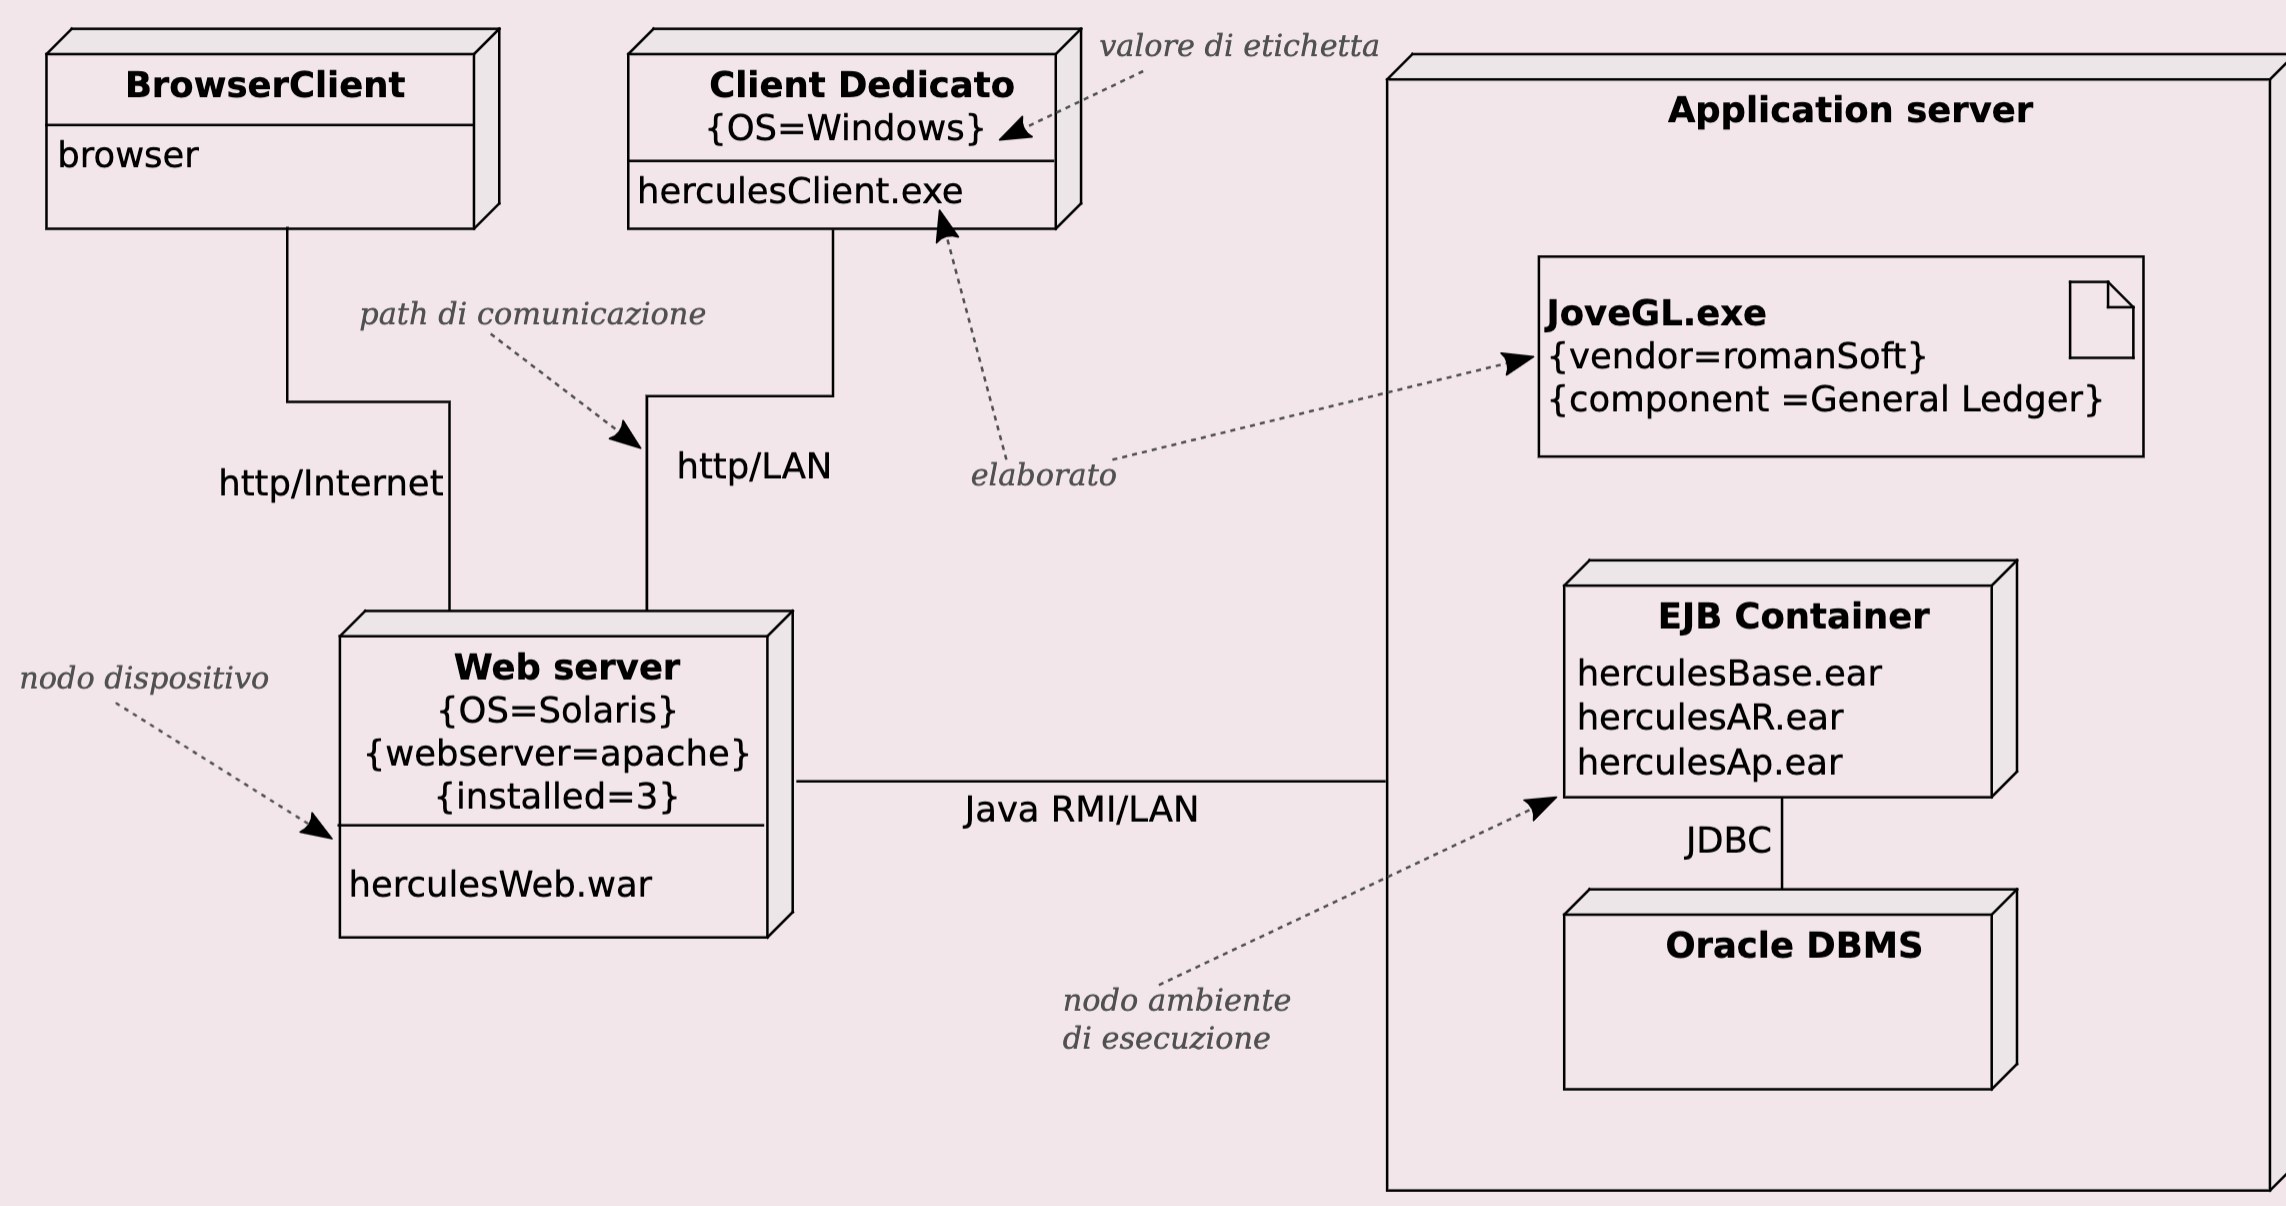
\includegraphics[width=1\linewidth]{assets/UML/deployment/deployment.png}
    \caption{Esempio di deployment diagram}
\end{figure}

\newpage
\newpage
\subsection{Object}

Gli \textbf{object diagram} rappresentano gli oggetti del sistema: specifiche di istanze di classi.

\paragraph{Oggetto} Rappresentato da box con la seguente intestazione:
\begin{center}
    $\langle$nomeOggetto$\rangle$ : $\langle$nomeClasse$\rangle$
\end{center}
Sono collegati tra loro da linee continue dette \textit{link 1-a-1} (istanze di associazioni).

\begin{figure}[H]
    \centering
    \subfloat[Class Diagram]{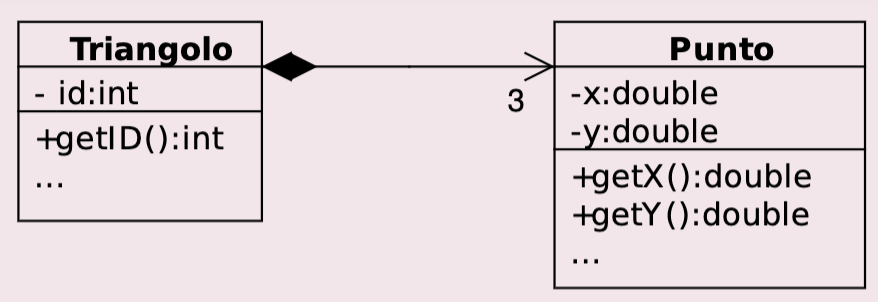
\includegraphics[width=0.6\linewidth]{assets/UML/class/class-2.png}}
    \hfill
    \subfloat[Object Diagram]{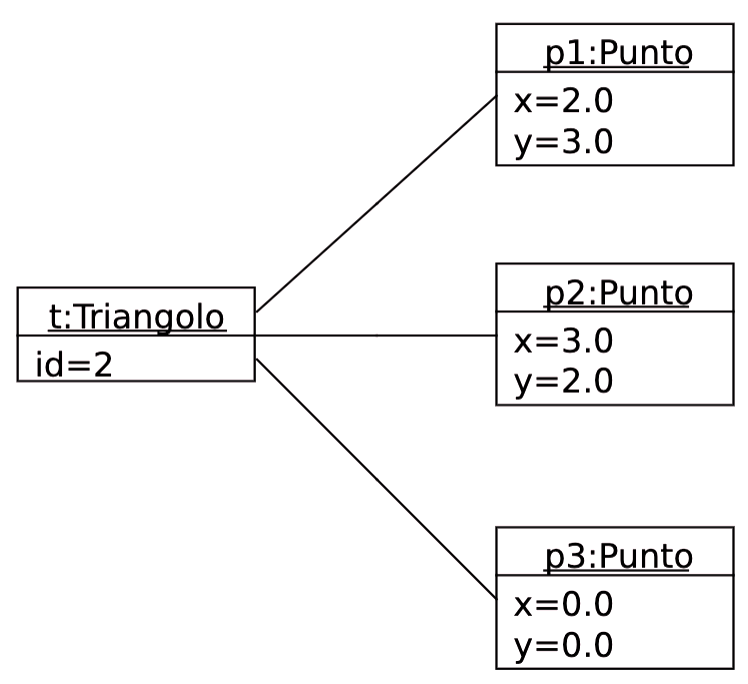
\includegraphics[width=0.3\linewidth]{assets/UML/object/object-1.png}}
    \caption{Differenze tra classi e oggetti in UML}
\end{figure}

\paragraph{Note} È possibile \textit{omettere degli attributi} oppure \textit{mostrare istanze di classi astratte}.

\paragraph{Relazioni} Nonostante il cambio di prospettiva dalle classi agli oggetti, le relazioni illustrate da un object diagram sono sempre di tipo \textit{statico}: il diagramma è una sorta di “fotografia congelata nel tempo”; mostra gli oggetti che costituiscono il sistema in un determinato momento.

\begin{figure}[H]
    \centering
    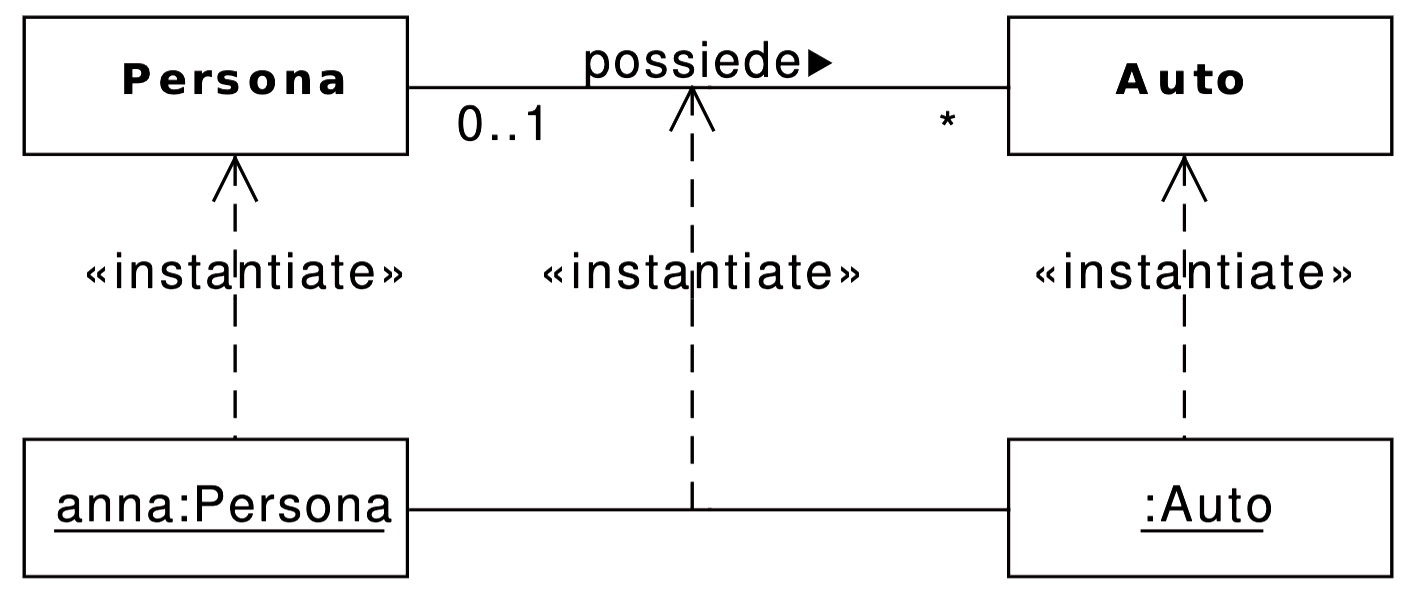
\includegraphics[width=0.75\linewidth]{assets/UML/object/object-2.png}
    \caption{La relazione di dipendenza $\langle$$\langle$instantiate$\rangle$$\rangle$ indica esplicitamente che gli oggetti sono istanze di classi ed il link è un'istanza della relazione \textit{possiede}.}
\end{figure}

\newpage
\subsection{Package}

\newpage
\subsection{Sequence}

\newpage
\subsection{State}

Lo \textbf{state diagram} descrive entità/oggetti il cui comportamento può cambiare dinamicamente nel tempo in relazione a determinati eventi o messaggi ricevuti.

Se la risposta dell'oggetto ad uno stimolo esterno non dipende unicamente dal suo stato corrente (valore dei campi), ma anche dalla sua storia (azioni passate eseguite in risposta a messaggi precedenti), si dice che l'oggetto possiede degli \textbf{stati di controllo}.

\paragraph{Automa a stati finiti} Se il numero di possibili risposte alle sollecitazioni è finito l'oggetto possiede un \textbf{automa a stati finiti} (es. iterator), ovvero un grafo orientato i cui nodi sono stati di controllo e i cui archi rappresentano le \textbf{transizioni di stato}.
Nell'approccio object-oriented un automa a stati finiti è associato a una classe e modella in maniera formale il comportamento delle sue istanze partendo da una specifica informale.

\paragraph{Stato iniziale} Lo stato di controllo in cui l'oggetto viene a trovarsi subito dopo la creazione: viene specificato tramite una \textbf{pseudo-transizione} che emana da un cerchietto nero (\textit{pseudo-stato}).

\paragraph{Stati finali} Nodi dai quali non si hanno transizione. Una transizione di stato è causata da un evento (\textit{trigger}). Si possono specificare delle \textbf{azioni} (operazioni atomiche non interrompibili). A seconda del modo distinguiamo fra:
\begin{itemize}

    \item \textbf{1. Automi di Mealy} in cui le azioni sono associate alle transizioni. Un'azione viene eseguita SEMPRE E SOLO in risposta al trigger della transizione a cui è associata;

    \item  \textbf{2. Automi di Moore} in cui le azioni sono associate agli stati. Un'azione viene eseguita quando l'automa si trova nello stato di controllo a cui è associata, a prescindere dalla transizione che ha portato in quello stato.

\end{itemize}


\begin{figure}[H]
    \centering
    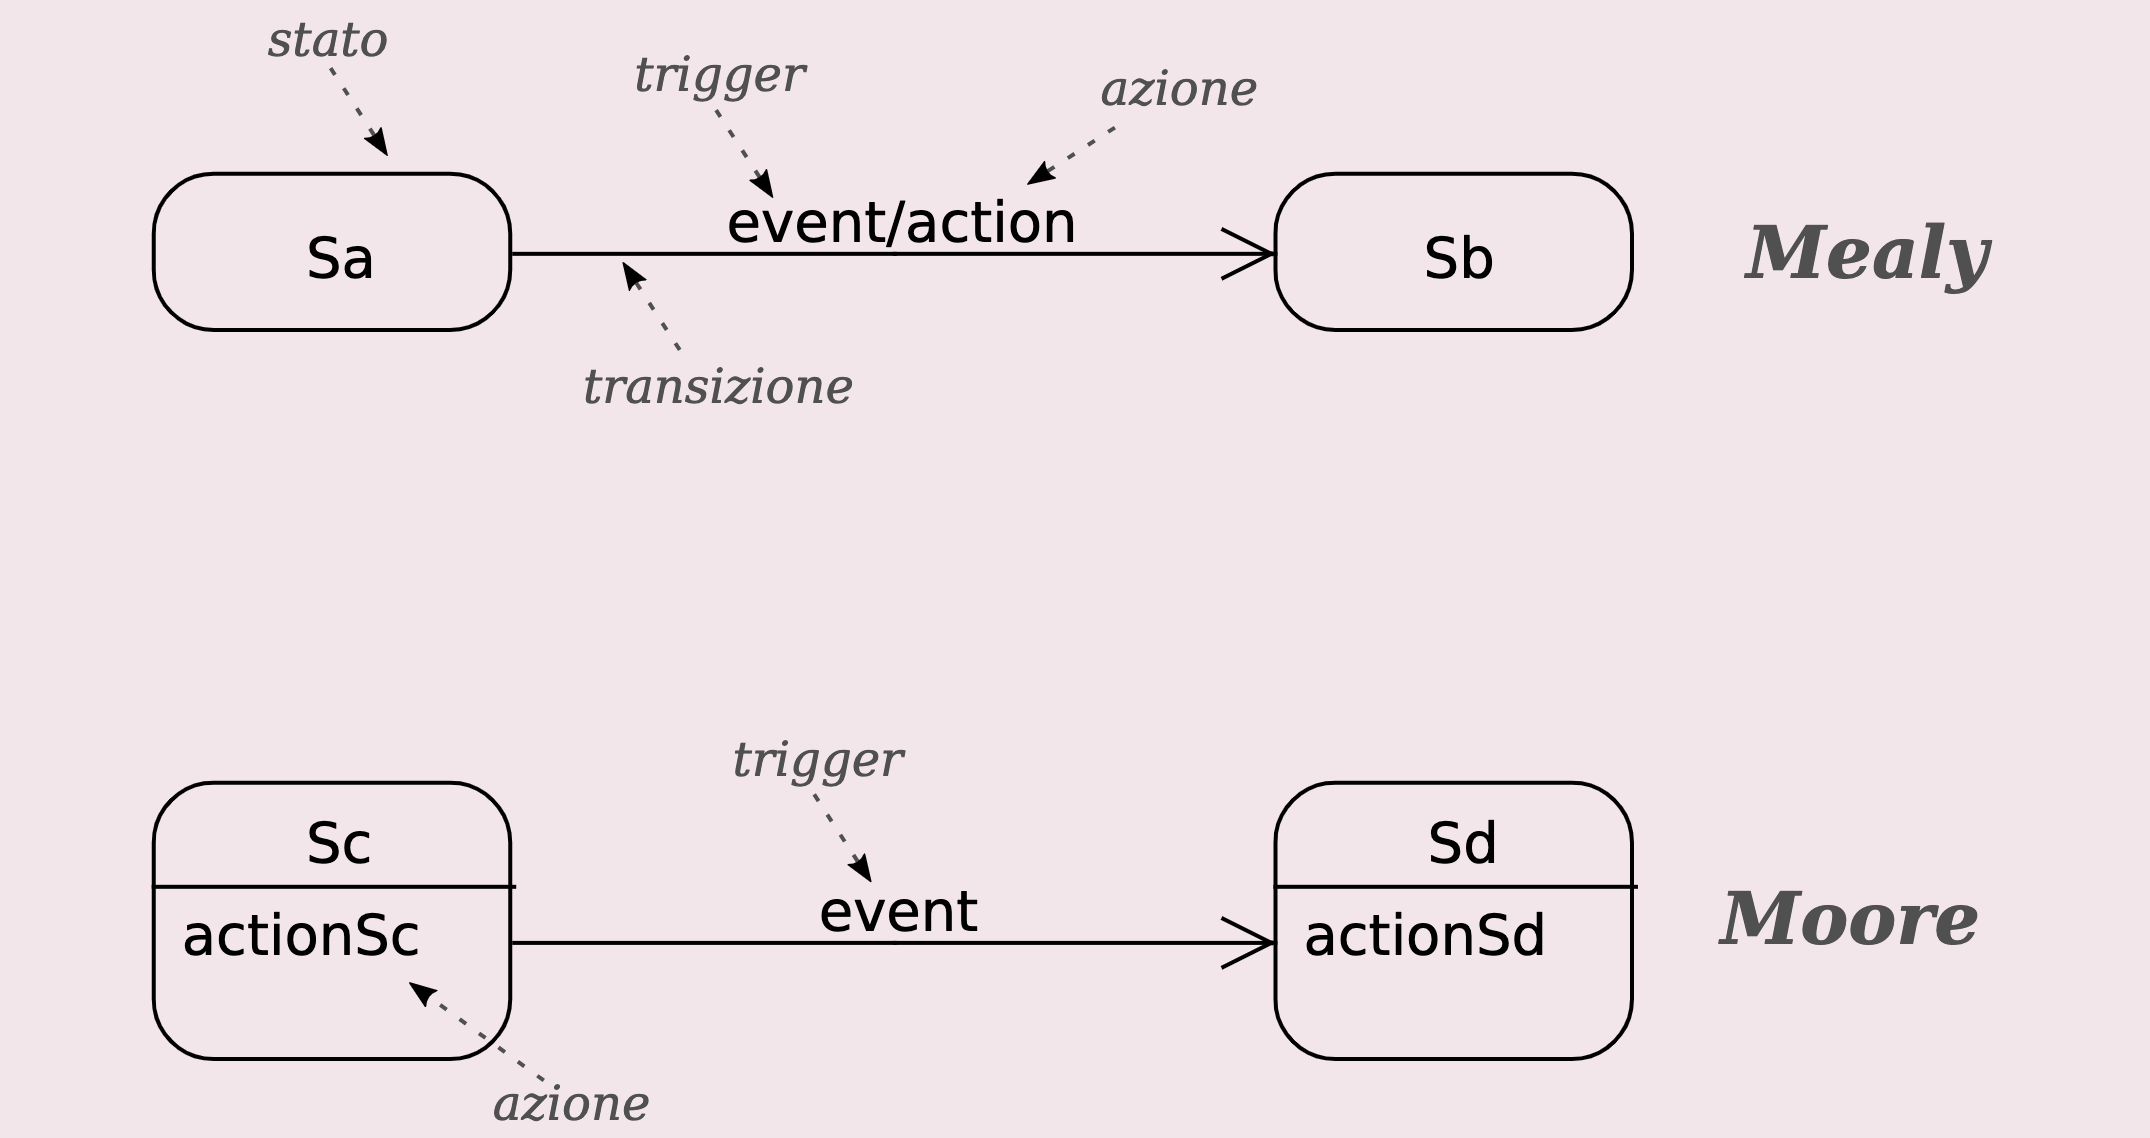
\includegraphics[width=0.75\linewidth]{assets/UML/state/state1.png}
\end{figure}

I due formalismi sono equivalenti: è sempre possibile trasformare un automa di Mealy in un automa di Moore e viceversa (il numero di stati potrebbe essere diverso).

\begin{figure}[H]
    \centering
    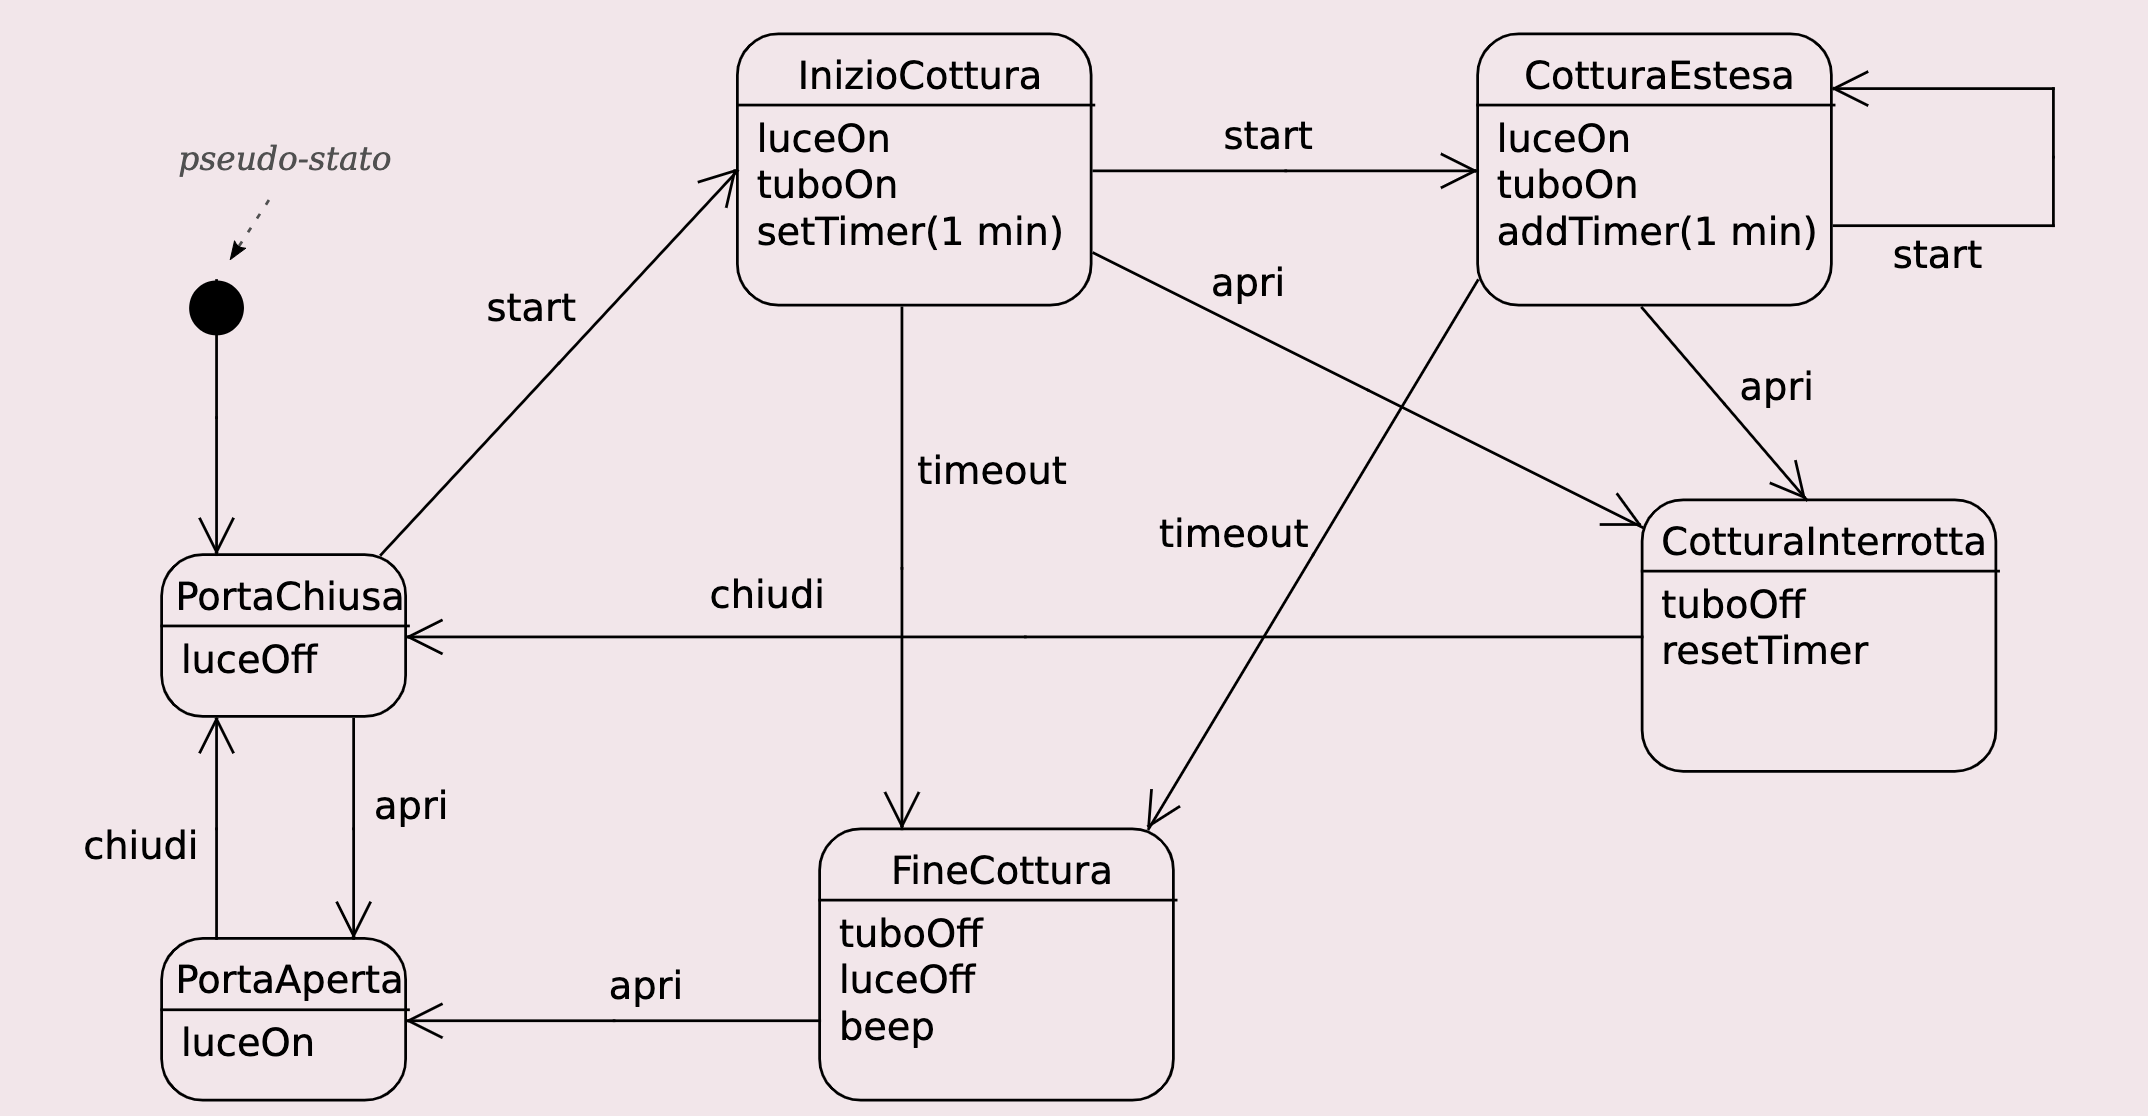
\includegraphics[width=0.75\linewidth]{assets/UML/state/state2.png}
    \caption{Esempio di automa: forno}
\end{figure}

\paragraph{State Chart} Sono una generalizzazione degli automi a stati finiti, rispetto ad essi consentono di modellare situazioni più complesse.

\begin{figure}[H]
    \centering
    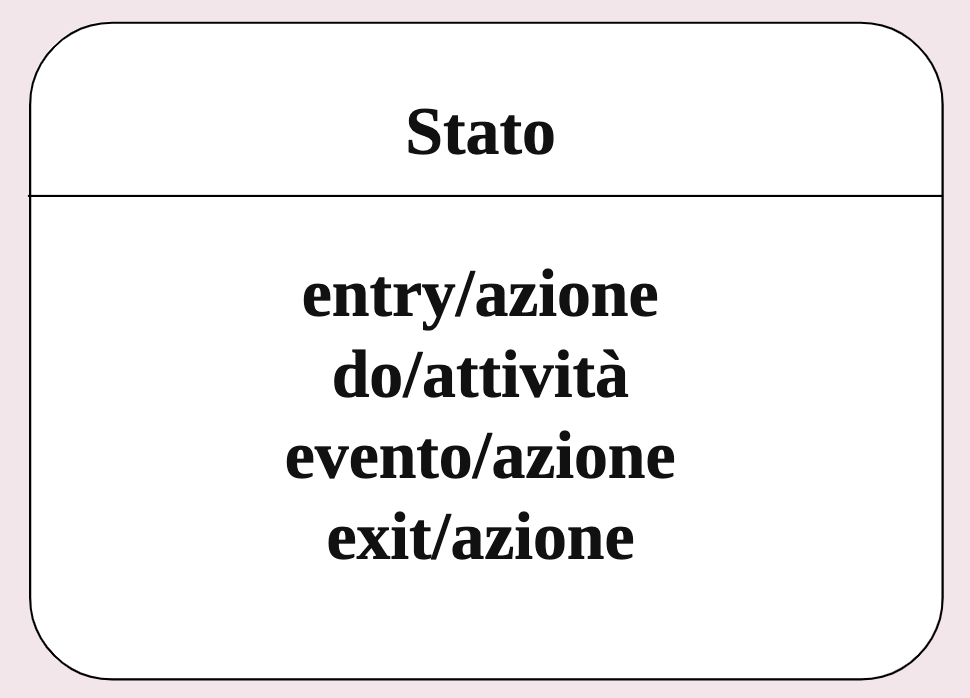
\includegraphics[width=0.25\linewidth]{assets/UML/state/state3.png}
    \caption{Rappresentazione di uno stato di controllo in uno state chart}
\end{figure}

\paragraph{Entry action} Azione triggerata entrando nello stato. Non va confusa con le \textit{attività interne} (non atomica, interrotta all'uscita dallo stato).

\paragraph{Exit action} Azione triggerata uscendo dallo stato. Si parla di \textit{transizione interna} quando l'oggetto esegue un'operazione rispetto ad un evento, ma senza uscire dallo stato. Si parla di \textit{transizione riflessiva} quando l'azione comporta il trigger di entrambe una entry action ed una exit action che riportano lo stato come era inizialmente (AUTOANELLO).

Gli state chart consentono di corredare i trigger con parametri e guardie (condizioni booleane in funzione dello stato corrente dell'oggetto e/o dei parametri ricevuti):

$$evento(parametro)\ \ [guardia]/azione$$

L'azione verrà eseguita se si verifica il trigger e se allo stesso tempo è vera la guardia. Fra le possibili azioni l'oggetto ha la facoltà di triggerare un altro oggetto (target).

$$send\ target.evento(parametri)$$

Scrivere dentro uno stato "evento/skip" specifica all'automa di ignorare il trigger quando si trova in quello stato.

Gli statechart consentono di modellare delle gerarchie annidando gli stati di controllo: ogni stato è contenuto in uno stato di livello gerarchico superiore (\textbf{\textit{superstato}}) che può a sua volta contenere più stati di livello gerarchico inferiore (\textbf{\textit{sottostati}}). Si dice \textbf{\textit{foglia}} uno stato privo di sottostati. Uno statechart in cui tutti gli stati sono sullo stesso piano gerarchico viene detto \textbf{\textit{piatto}}.

\begin{figure}[H]
    \centering
    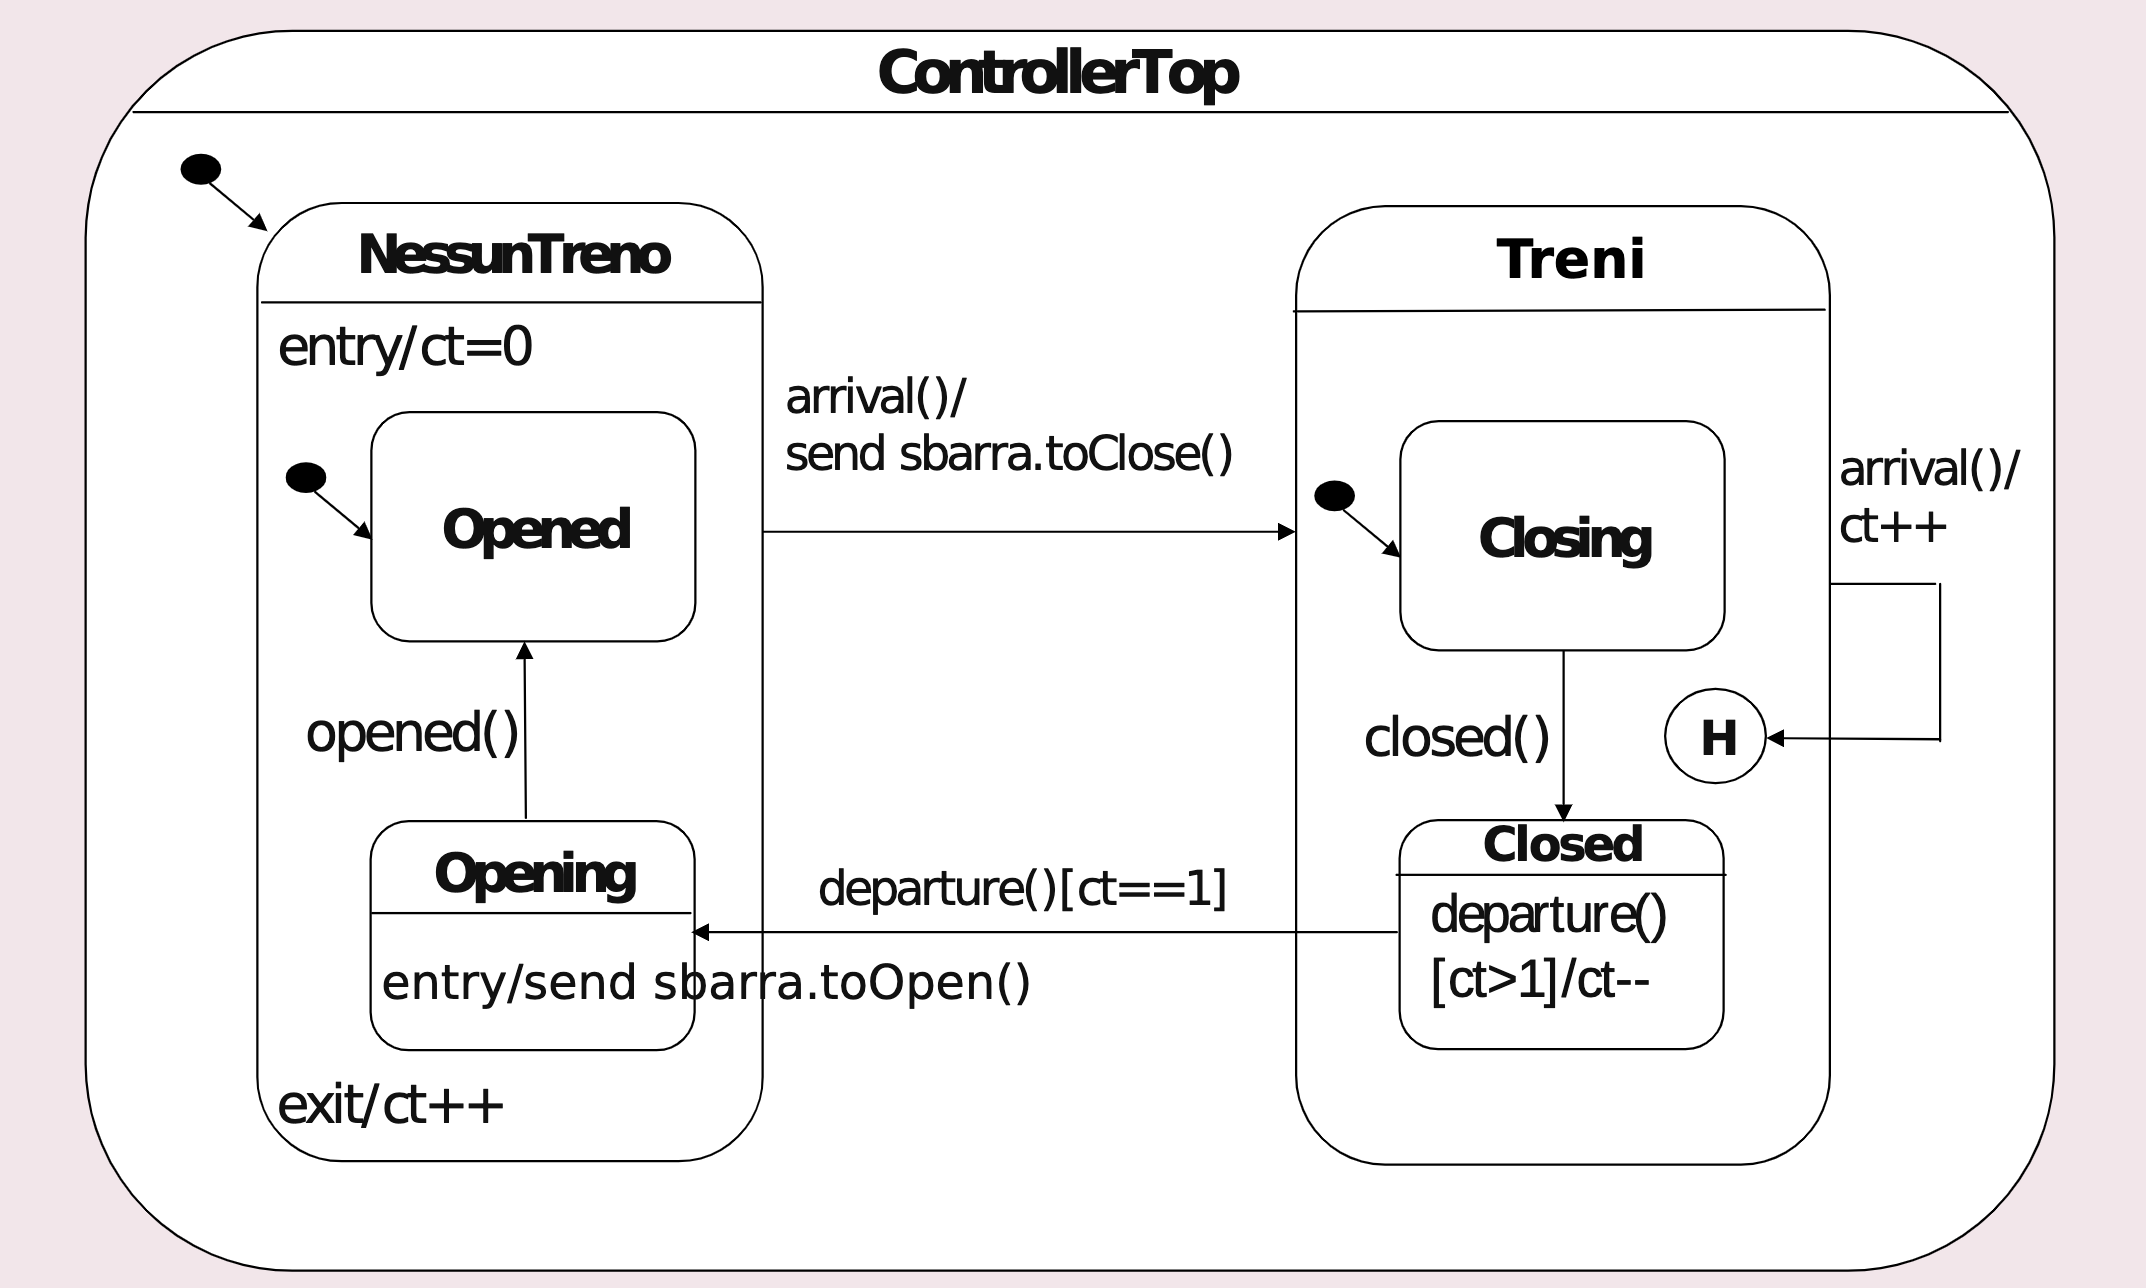
\includegraphics[width=0.75\linewidth]{assets/UML/state/state4.png}
    \caption{Esempio di state chart: controller di un treno}
\end{figure}

Per ogni stato non foglia una pseudo-transizione indica qual è il sottostato iniziale. Si definisce "configurazione" dell'automa il percorso che va dallo stato di più alto livello gerarchico fino allo stato foglia attuale. Nell'esempio, la configurazione iniziale dell'automa è la seguente:

$$ControllerTop.NessunTreno.0pened$$

\paragraph{OR-decomposition} Lo stato foglia attuale è sufficiente a definire univocamente la configurazione corrente dell'automa. Questo perché si è applicato il \textbf{principio dell'OR esclusivo} (XOR): in ogni stato NON foglia, l'automa deve trovarsi in uno e uno solo dei ossibili sottostati.

Si definisce \textbf{transizione di gruppo} quella che parte da uno stato non foglia: può essere triggerata a presciendere dal sottostato specifico in cui si trova l'automa. 

Un \textbf{connettore di storia} è un elemento posto all'interno di uno stato di controllo per consentire all'automa di memorizzare, quando si trova in quello stato, la configurazione corrente. Tornando nello stato l'automa non assumerà la configurazione di default, bensì quella memorizzata nel connettore. Esistono due tipi di connettori di storia:
\begin{itemize}
    \item \textbf{Storia superficiale (H)}: memorizzano la configurazione dallo stato di livello gerarchico più alto fino al livello dei sottostati dello stato con il connettore;
    \item \textbf{Storia profonda (H*)}: memorizzano la configurazione dallo stato di livello gerarchico più alto fino allo stato foglia corrente, dunque scendendo in profondità oltre i sottostati dello stato contenente il connettore.
\end{itemize}

\begin{figure}[H]
    \centering
    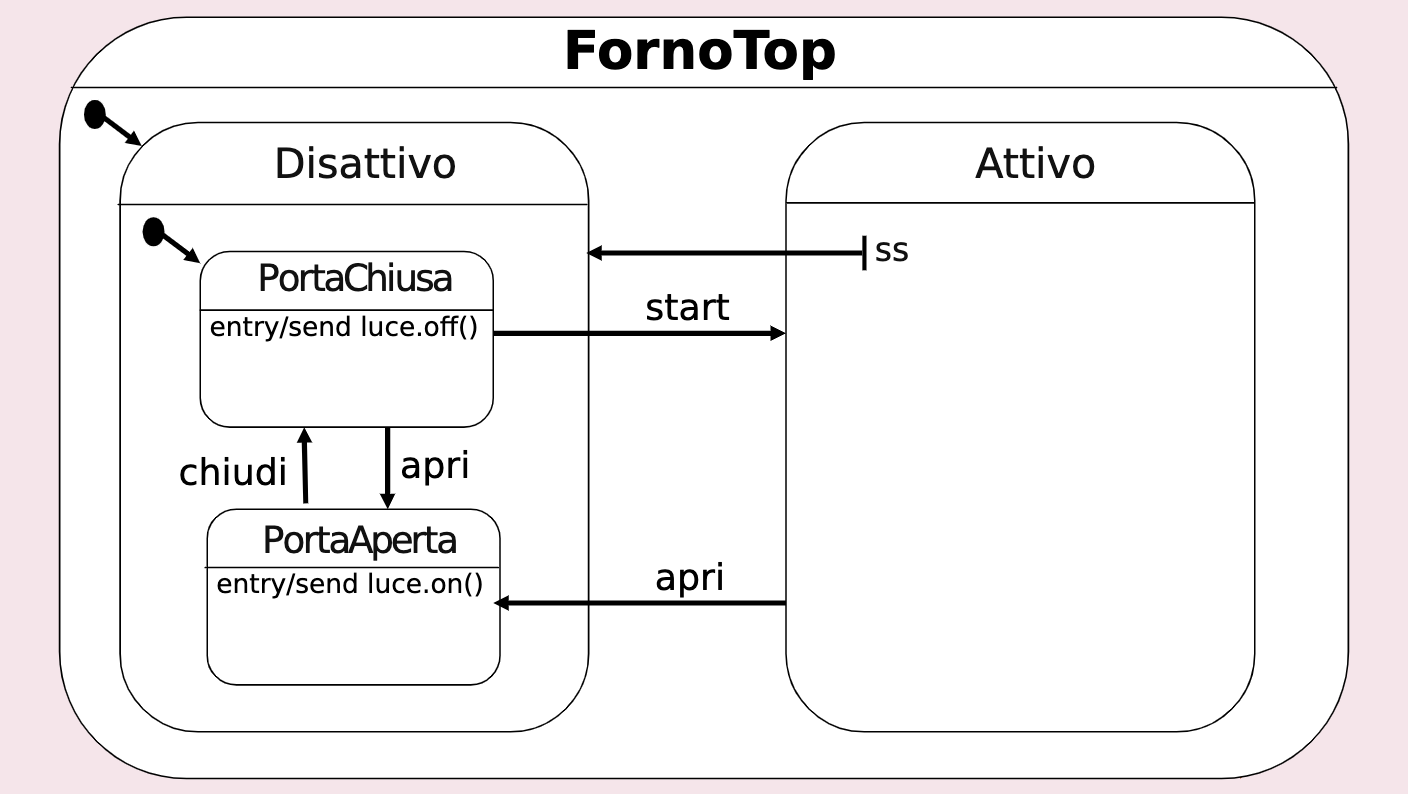
\includegraphics[width=0.75\linewidth]{assets/UML/state/state5.png}
    \caption{Esempio di statechart per il Forno}
\end{figure}

\begin{figure}[H]
    \centering
    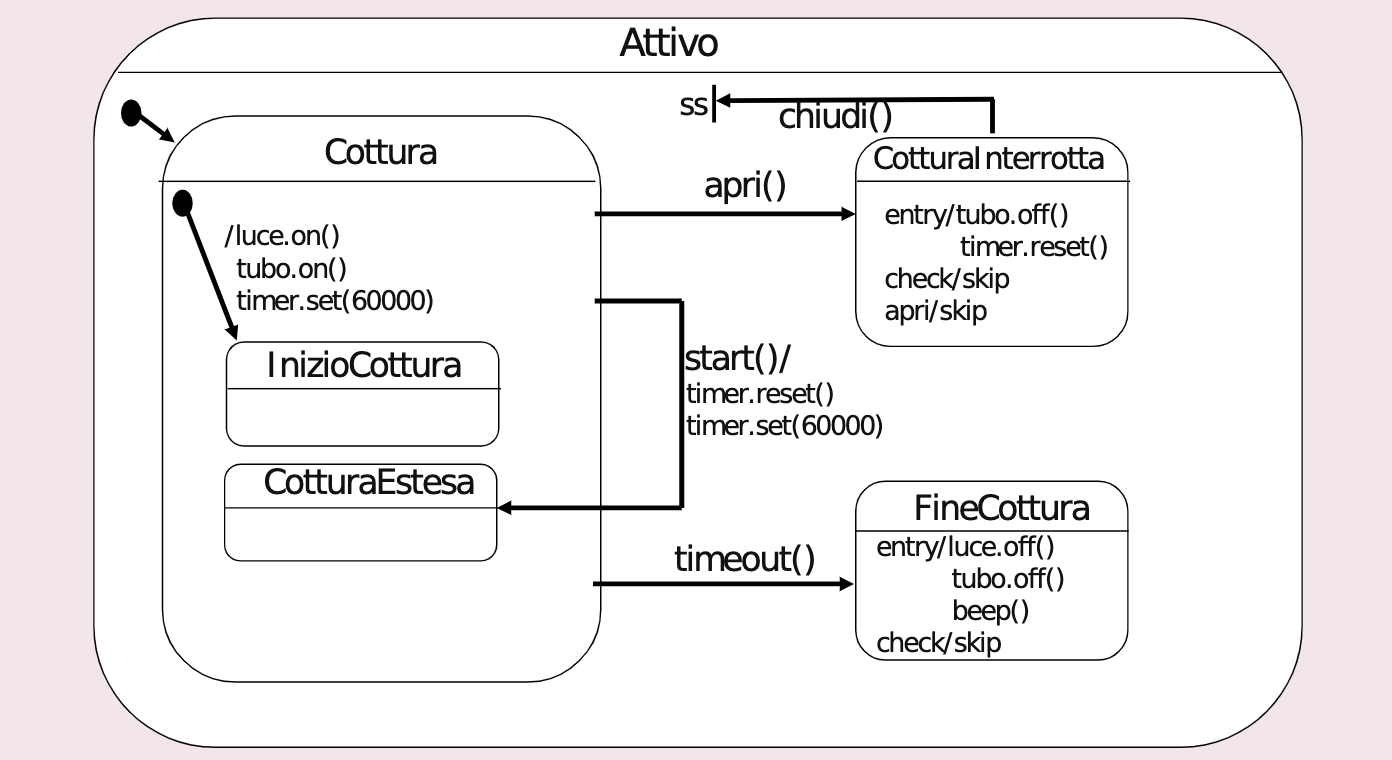
\includegraphics[width=0.75\linewidth]{assets/UML/state/state6.png}
    \caption{Definizione del macrostato "Attivo"}
\end{figure}

\begin{figure}[H]
    \centering
    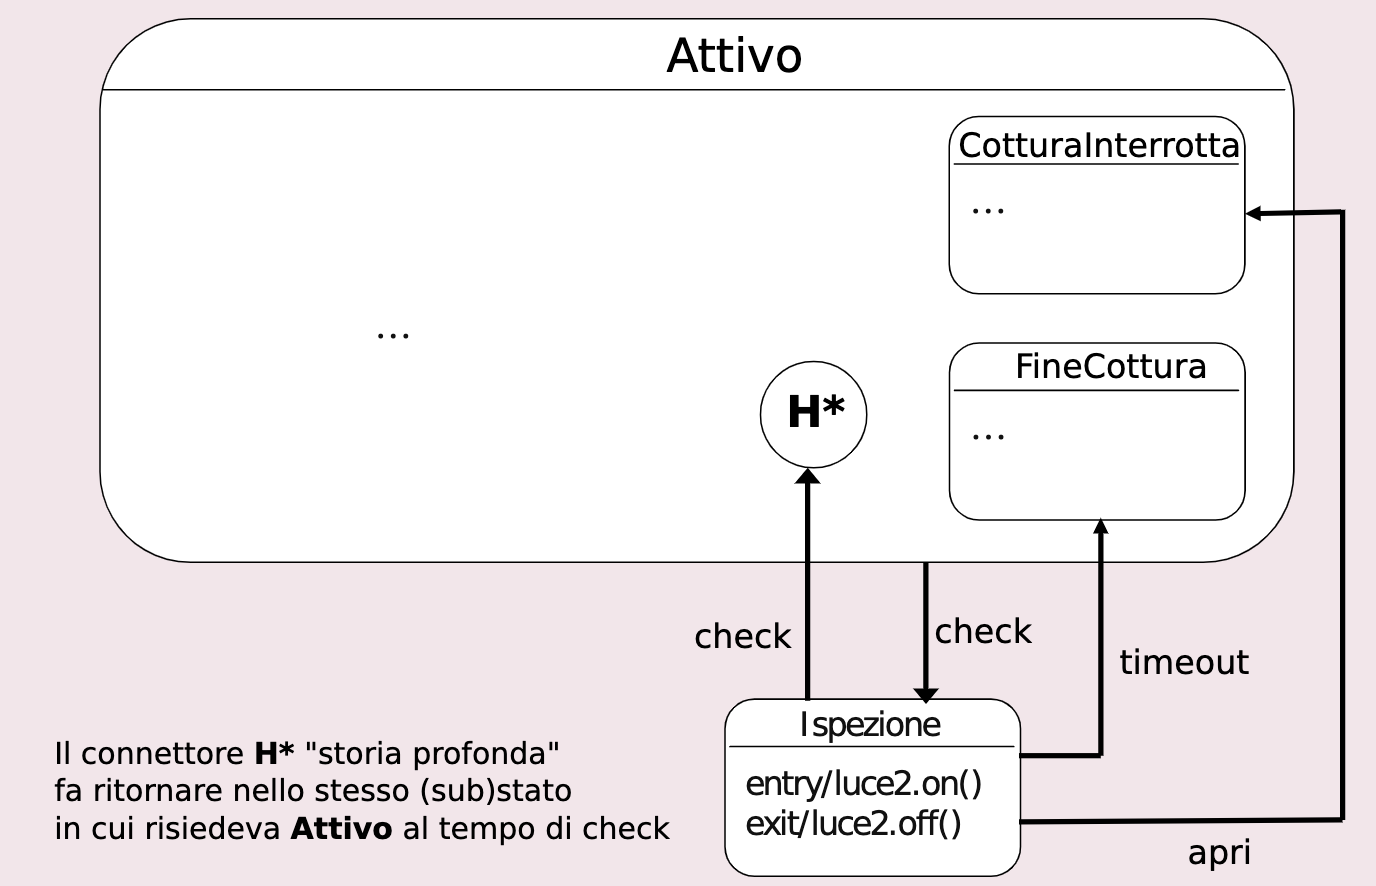
\includegraphics[width=0.75\linewidth]{assets/UML/state/state7.png}
    \caption{Esempio di stato ispezione}
\end{figure}

In generale i connettori di storia dovrebbero avere anche una transizione uscente verso un sottostato del macrostato in cui sono contenuti, in modo da poter essere attivati quando l'automa si trova in quello stato. In sua assenza e in assenza di memoria si raggiunge lo stato di default.

Sfruttando il principio di modularità, è possibile definire la gerarchia di uno solo dei possibili stati di controllo, astraendo dai dettagli interni degli altri stati. La presenza di stati non ancora definiti che sono punto di partenza/arrivo di transizioni è segnalata con un cosiddetto \textbf{state stub}.

\paragraph{Nota} Per via del concetto di configurazione, in una transizione di stato è necessario individuare:

\begin{itemize}
    \item \textbf{Exit path}: elenco degli stati di controllo da cui si esce, partendo dallo stato sorgente della transizione e risalendo fino al \textbf{Minimum Common Ancestor} (MCA) con lo stato di destinazione (MCA escluso). Si devono eseguire exit action di tutti gli stati attraversati.
    \item \textbf{Entry path}: elenco degli stati di controllo in cui si entra, partendo dall'MCA (escluso) e scendendo fino allo stato destinazione della transizione. Si devono eseguire tutte le entry action degli stati attraversati.
\end{itemize}

L'MCA è il superstato di livello gerarchico più piccolo che contenga sia la destinazione che la sorgente della transizione.

\subsubsection{Estendere lo state diagram}

Si possono includere negli statechart elementi tipici di un activity diagram: es. punti decisionali (rombi) che pongono due o più transizioni in alternativa. Si può introdurre un'attività (non atomica, interrompibile) in uno stato dcon la sintassi:

$$do:activity_name$$

Uno stato con una attività interna o con eventi processati localmente allo stato può essere scomposto in più sottostati. È possibile triggerare una transizione non con un evento esterno, bensì tramite la maturazione di una condizione internamente all'oggetto:

$$when condition$$

Ancora, il trigger della transizione potrebbe essere un \textit{evento di tempo}:

$$after time_expression$$


\paragraph{AND-decomposition} Lo stato foglia attuale NON è sufficiente a definire univocamente la condizione corrente dell'automa. In ogni stato NON foglia, l'automa può trovarsi contemporaneamente in due o più possibili sottostati. Lo stato viene diviso in \textit{regioni} parallele e concorrenti.

\begin{figure}[H]
    \centering
    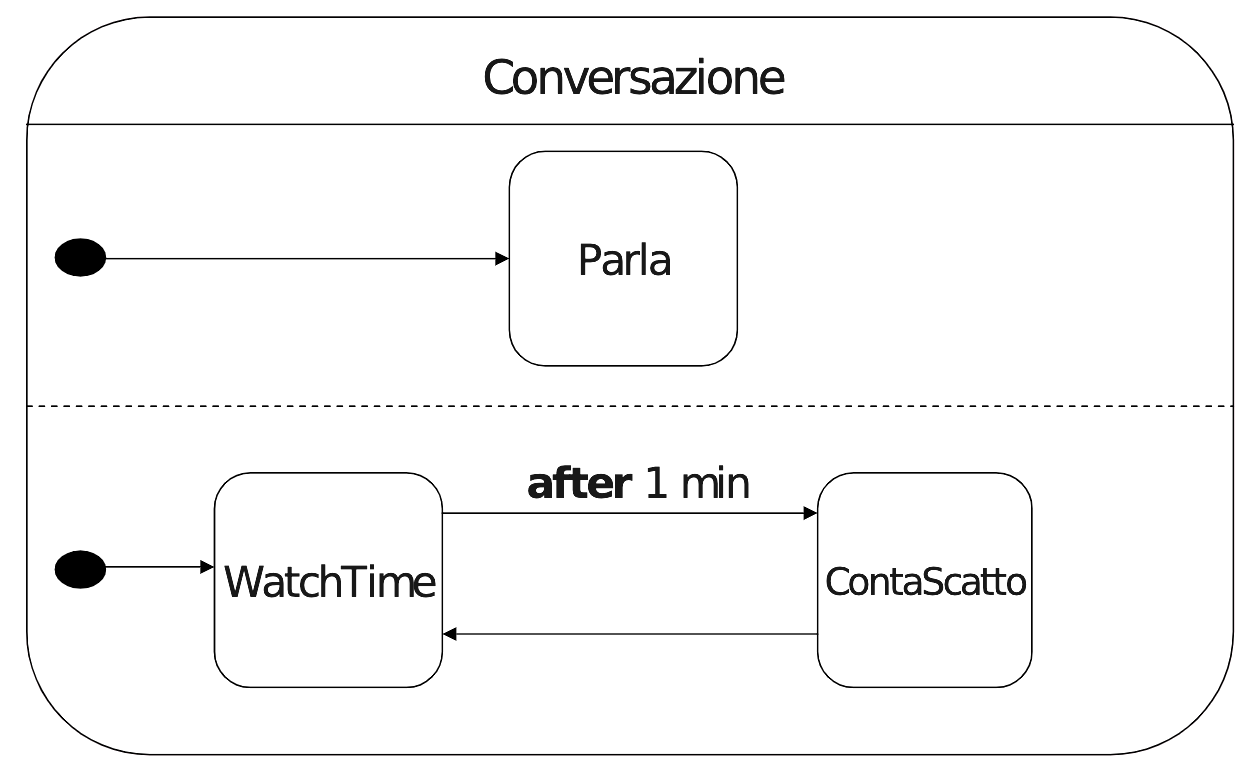
\includegraphics[width=0.75\linewidth]{assets/UML/state/state8.png}
\end{figure}

Nell'esempio, la configurazione inziale è:

$$Conversazione.Parla|WatchTime$$ 

Sottostati paralleli implicano l'esistenza di thread multipli in uno stesso oggetto (occorre adottare meccanismi di mutua esclusione per proteggere i dati condivisi).

Le transizioni nei due stati paralleli possono essere sincronizzate introducendo delle \textbf{barre di sincronizzazione} e degli \textbf{pseudo-stati di sincronismo} (synch state): l'avanzamento in un sottostato può awenire solo se nello stato parallelo si è raggiunto un certo punto.

\begin{figure}[H]
    \centering
    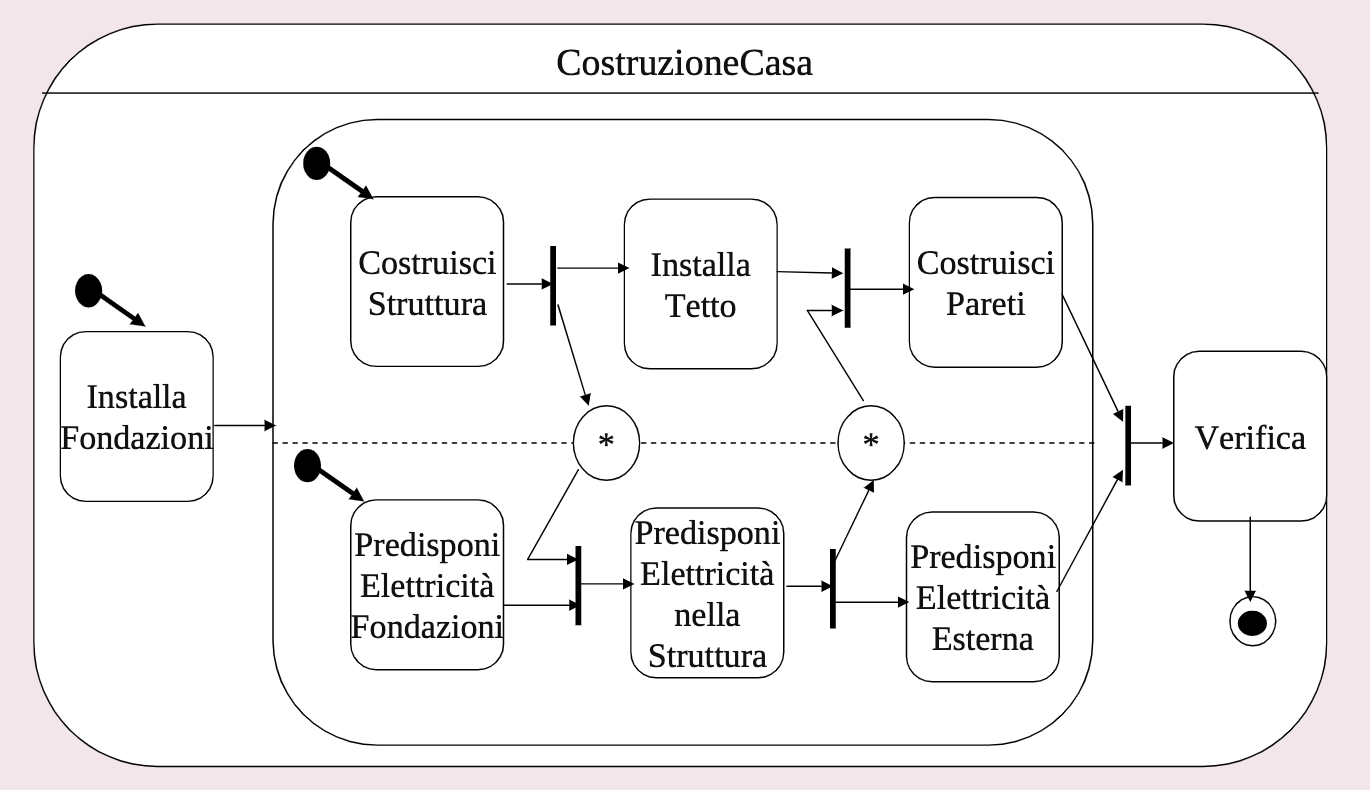
\includegraphics[width=0.75\linewidth]{assets/UML/state/state9.png}
\end{figure}

\newpage
\subsection{Structure Composite}

Lo \textbf{structure composite diagram} consente di scomporre gerarchicamente una classe sulla base dei suoi contenuti (interfacce richieste e fornite) e di mostrare la composizione interna delle sue istanze. Illustra le dipendenze dinamiche fra gli oggetti che compongono il sistema.

\begin{figure}[H]
    \centering
    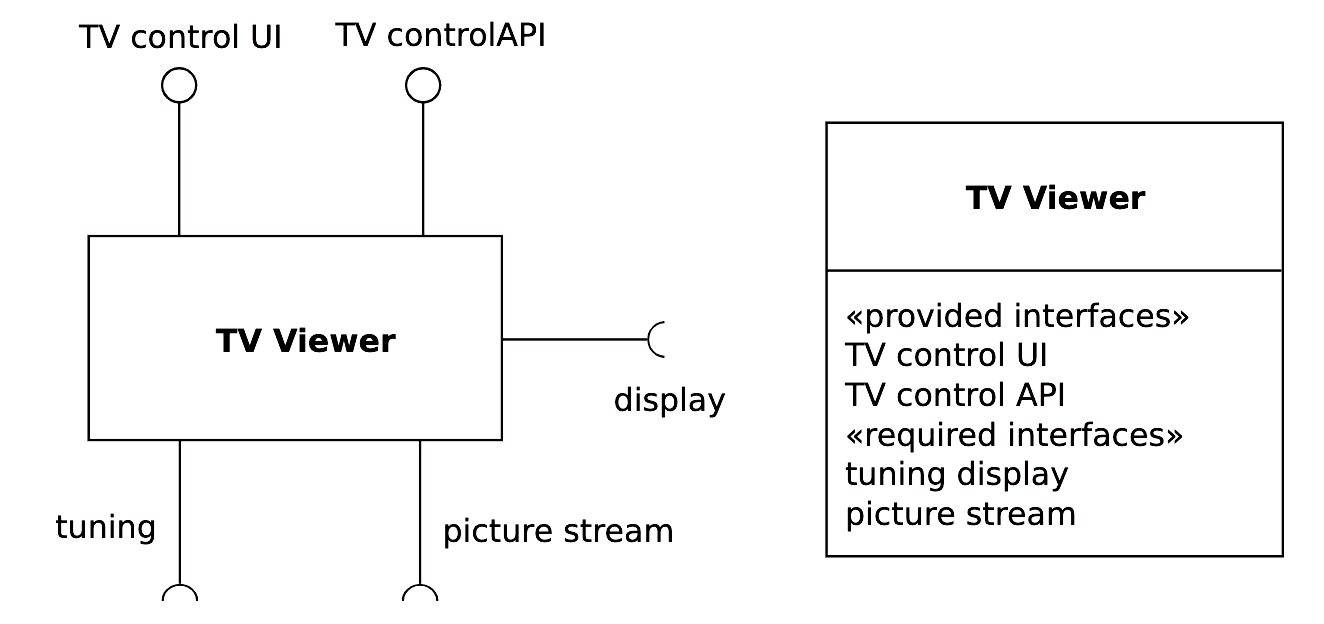
\includegraphics[width=0.75\linewidth]{assets/UML/struct_comp/struct_comp.png}
    \caption{Struttura interna della classe; le interfacce richieste/fornite sono raggruppate logicamente tramite "porte".}
\end{figure}

\paragraph{Esempio} TV Viewer: ogni istanza possiede un'istanza di TVPresenter e un'istanza di Generator (campi dell'oggetto), attraverso le quali fornisce e richiede determinate interfacce. Ogni proprietà posseduta dalla classe è una parte dell'istanza, indicata da \textbf{nome:classe} e dalla molteplicità. Le varie parti sono collegate da \textbf{connettori} (linee continue). I \textbf{connettori di delega} (frecce tratteggiate a punta aperta) collegano una parte alle interfacce che fornisce o richiede.

\begin{figure}[H]
    \centering
    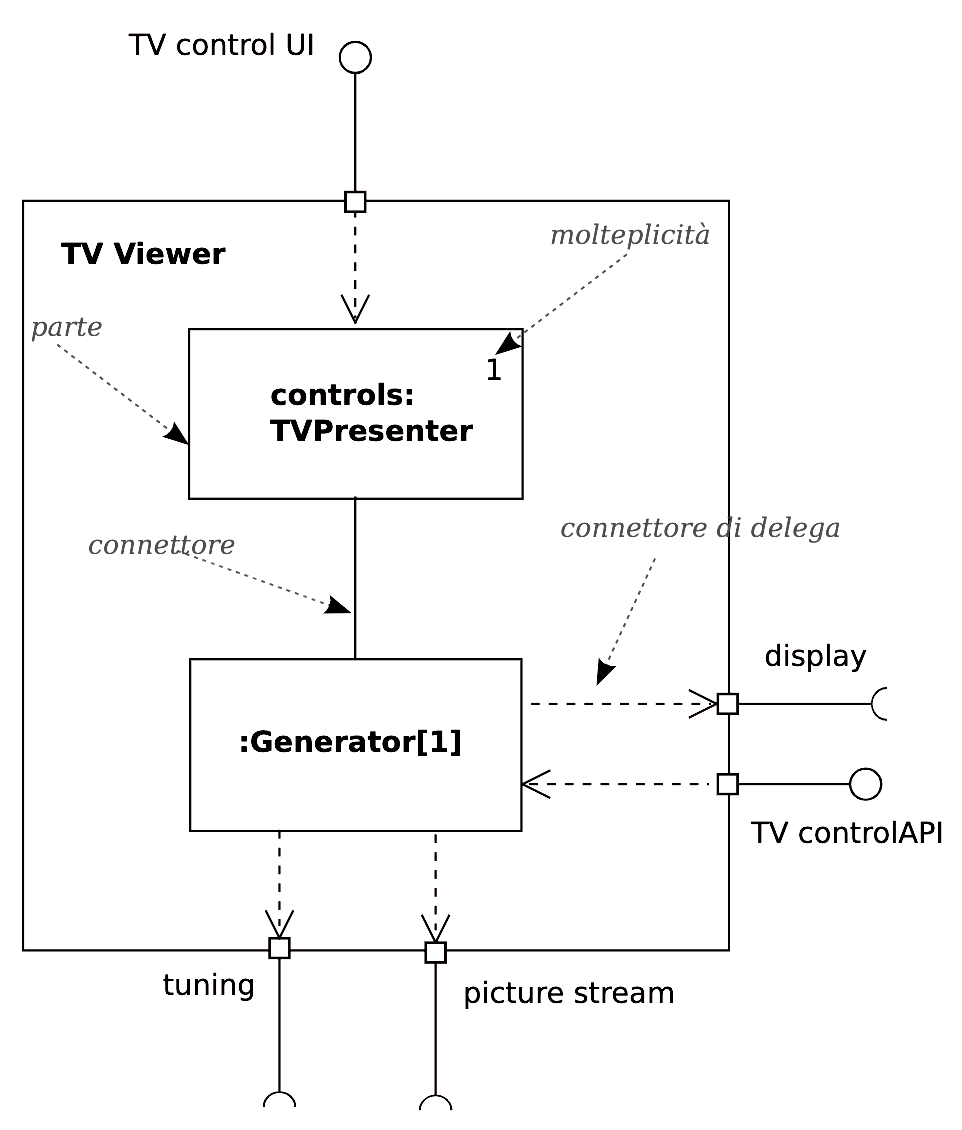
\includegraphics[width=0.4\linewidth]{assets/UML/struct_comp/struct_comp2.png}
    \caption{Esempio di structure composite (TV Viewer)}
\end{figure}

\newpage
\subsection{UseCase}

Gli \textbf{UseCase Diagram} servono per identificare le funzionalità svolte dal sistema software. Queste devono essere assegnate ad oggetti/classi (\textbf{assegnazione di responsabilità}). Si parte dalle macro-funzionalità, raffinandole fino ad arrivare ad operazioni che non ammettono decomposizione. Eventuali ambiguità possono essere chiarite tramite \textit{Activity Diagram}. L'analisi dei casi d'uso può:
\begin{itemize}
    \item aiutare ad identificare gli oggetti
    \item definire i casi di test di moduli
    \item descrivere le dinamiche di interazione con il sistema
\end{itemize}

\begin{figure}[H]
    \centering
    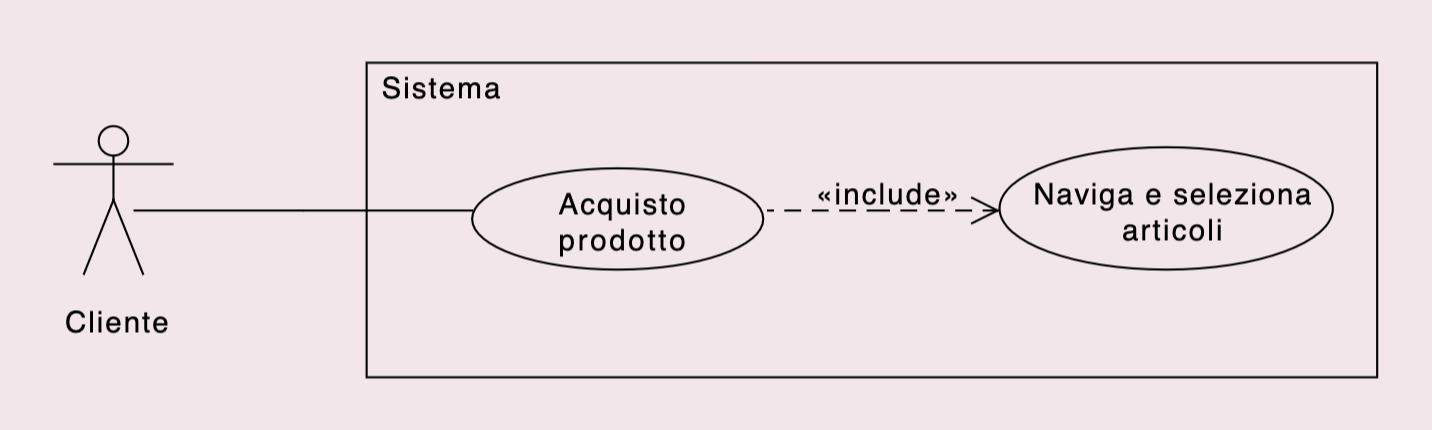
\includegraphics[width=0.75\linewidth]{assets/UML/use-case/use-case1.png}
    \caption{Esempio di UseCase Diagram}
    \label{fig:use-case1}
\end{figure}

\paragraph{Attore} Rappresenta un ruolo interpretato da entità esterne (utenti o sistemi). L'\textbf{attore principale} è colui che persegue lo scopo del caso d'uso (gli altri sono secondari). Sussiste una relazione molti-a-molti tra attori e casi d'uso.

\textbf{\textit{Rappresentazione}}: omino stilizzato.

\paragraph{Scenario} Sequenza di passi che caratterizza l'interazione complessa tra un attore ed il sistema software stesso. In particolare si distinguono:
\begin{itemize}
    \item \textbf{Main scenario}: scenario principale di successo (obiettivo raggiunto)
    \item \textbf{Scenari secondari} (o estensioni del main): divergono dal main scenario o sono contenuti in esso (possono o meno raggiungere lo scopo prefissato)
\end{itemize}
\textbf{\textit{Rappresentazione}}: rettangolo contenente i casi d'uso dello scopo.

\paragraph{Caso d'uso} Insieme di scenari che hanno lo stesso scopo finale (per l'utente). Uno scenario è una possibile "esecuzione" (istanza) del caso d'uso. Può comprendere:
\begin{itemize}
    \item \textbf{Pre-condizioni}: descrivono ciò che il sistema deve assicurarsi prima che il caso d'uso possa avere inizio
    \item \textbf{Garanzie}: descrivono ciò che il sistema deve assicurarsi alla fine dello svolgimento del caso d'uso
    \item \textbf{Trigger}: specificano l'evento che da origine al caso d'uso
\end{itemize}
\textit{Alastair Cockburn} suddivide i casi d'uso in tre livelli:
\begin{itemize}
    \item \textbf{Kite-level}: mostrano come più sea-level portano all'interazione tra diversi attori (livello superficiale)
    \item \textbf{Sea-level}: interazioni attore principale/sistema (livello mediano)
    \item \textbf{Fish-level}: esistono perché inclusi in un sea-level (livello profondo)
\end{itemize}
Un passo di caso d'uso corrisponde ad un'interazione tra attore e sistema; è descritto da una frase semplice e non esprime dettagli tecnici.

\textbf{\textit{Rappresentazione}}: ellisse contenente il nome del caso d'uso.

\begin{figure}[H]
  \centering
  \subfloat[Generalizzazione tra casi d'uso, il caso d'uso figlio "specializza" (estende) alcuni aspetti del padre]{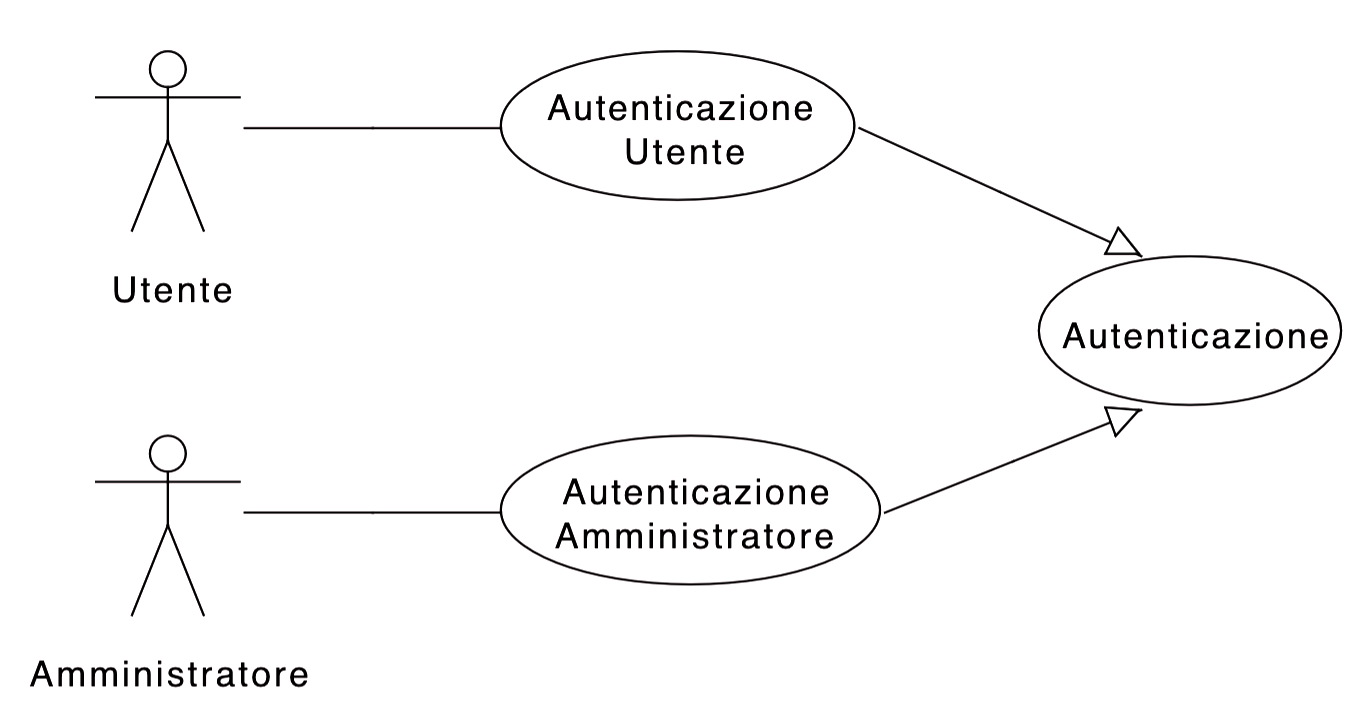
\includegraphics[width=0.575\linewidth]{assets/UML/use-case/use-case2.png}}
  \hfill
  \subfloat[Generalizzazione tra attori, ruolo figlio più specifico, \textit{compatibile} con il ruolo padre]{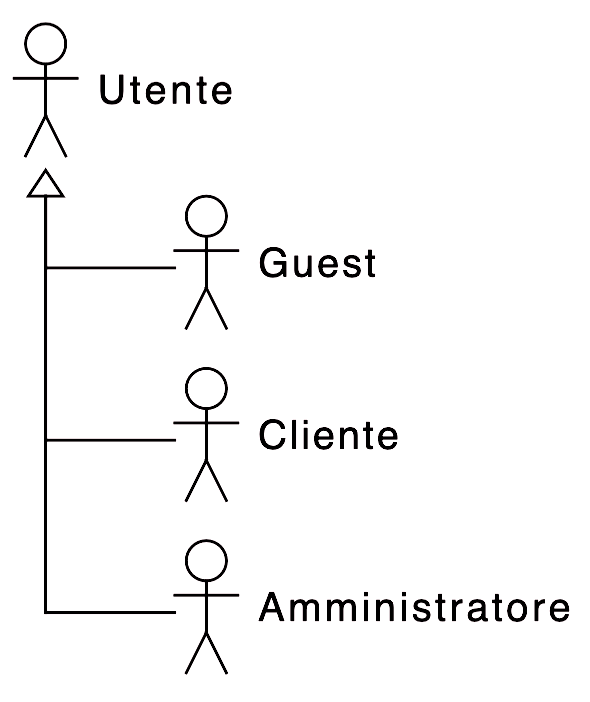
\includegraphics[width=0.25\linewidth]{assets/UML/use-case/use-case3.png}}
\end{figure}

\subparagraph{Estensione} Condizione che determina il verificarsi di interazioni diverse dallo scenario principale. Si indicano: il passo in cui si verifica la condizione, i passi (numerati) che descrivono le interazioni dell'estensione e (se necessario) il punto di rientro nello scenario principale.
\textbf{\textit{Rappresentazione}}: linea tratteggiata che termina con una freccia etichettata con la parola chiave $\langle\langle$extend$\rangle\rangle$

\begin{figure}[H]
  \centering
  \subfloat[Relazione di estensione]{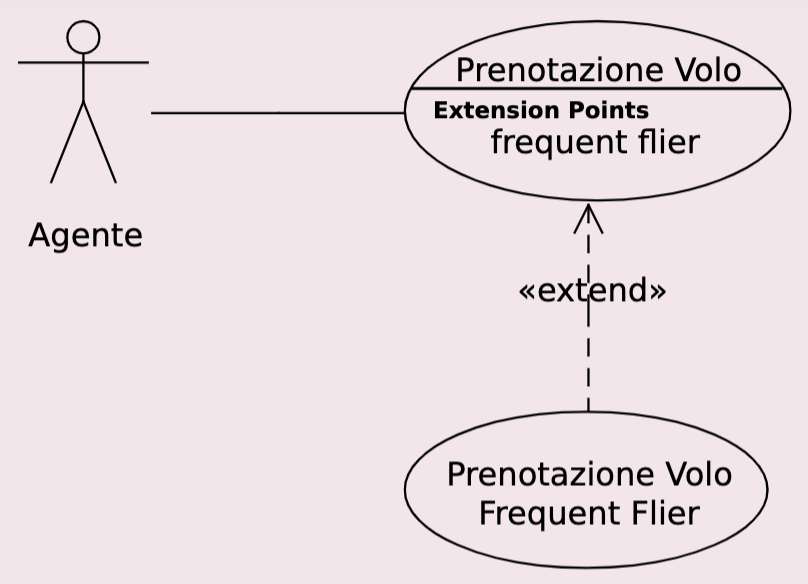
\includegraphics[width=0.41\linewidth]{assets/UML/use-case/use-case5.png}}
  \hfill
  \subfloat[Esempio di caso d'uso in forma testuale]{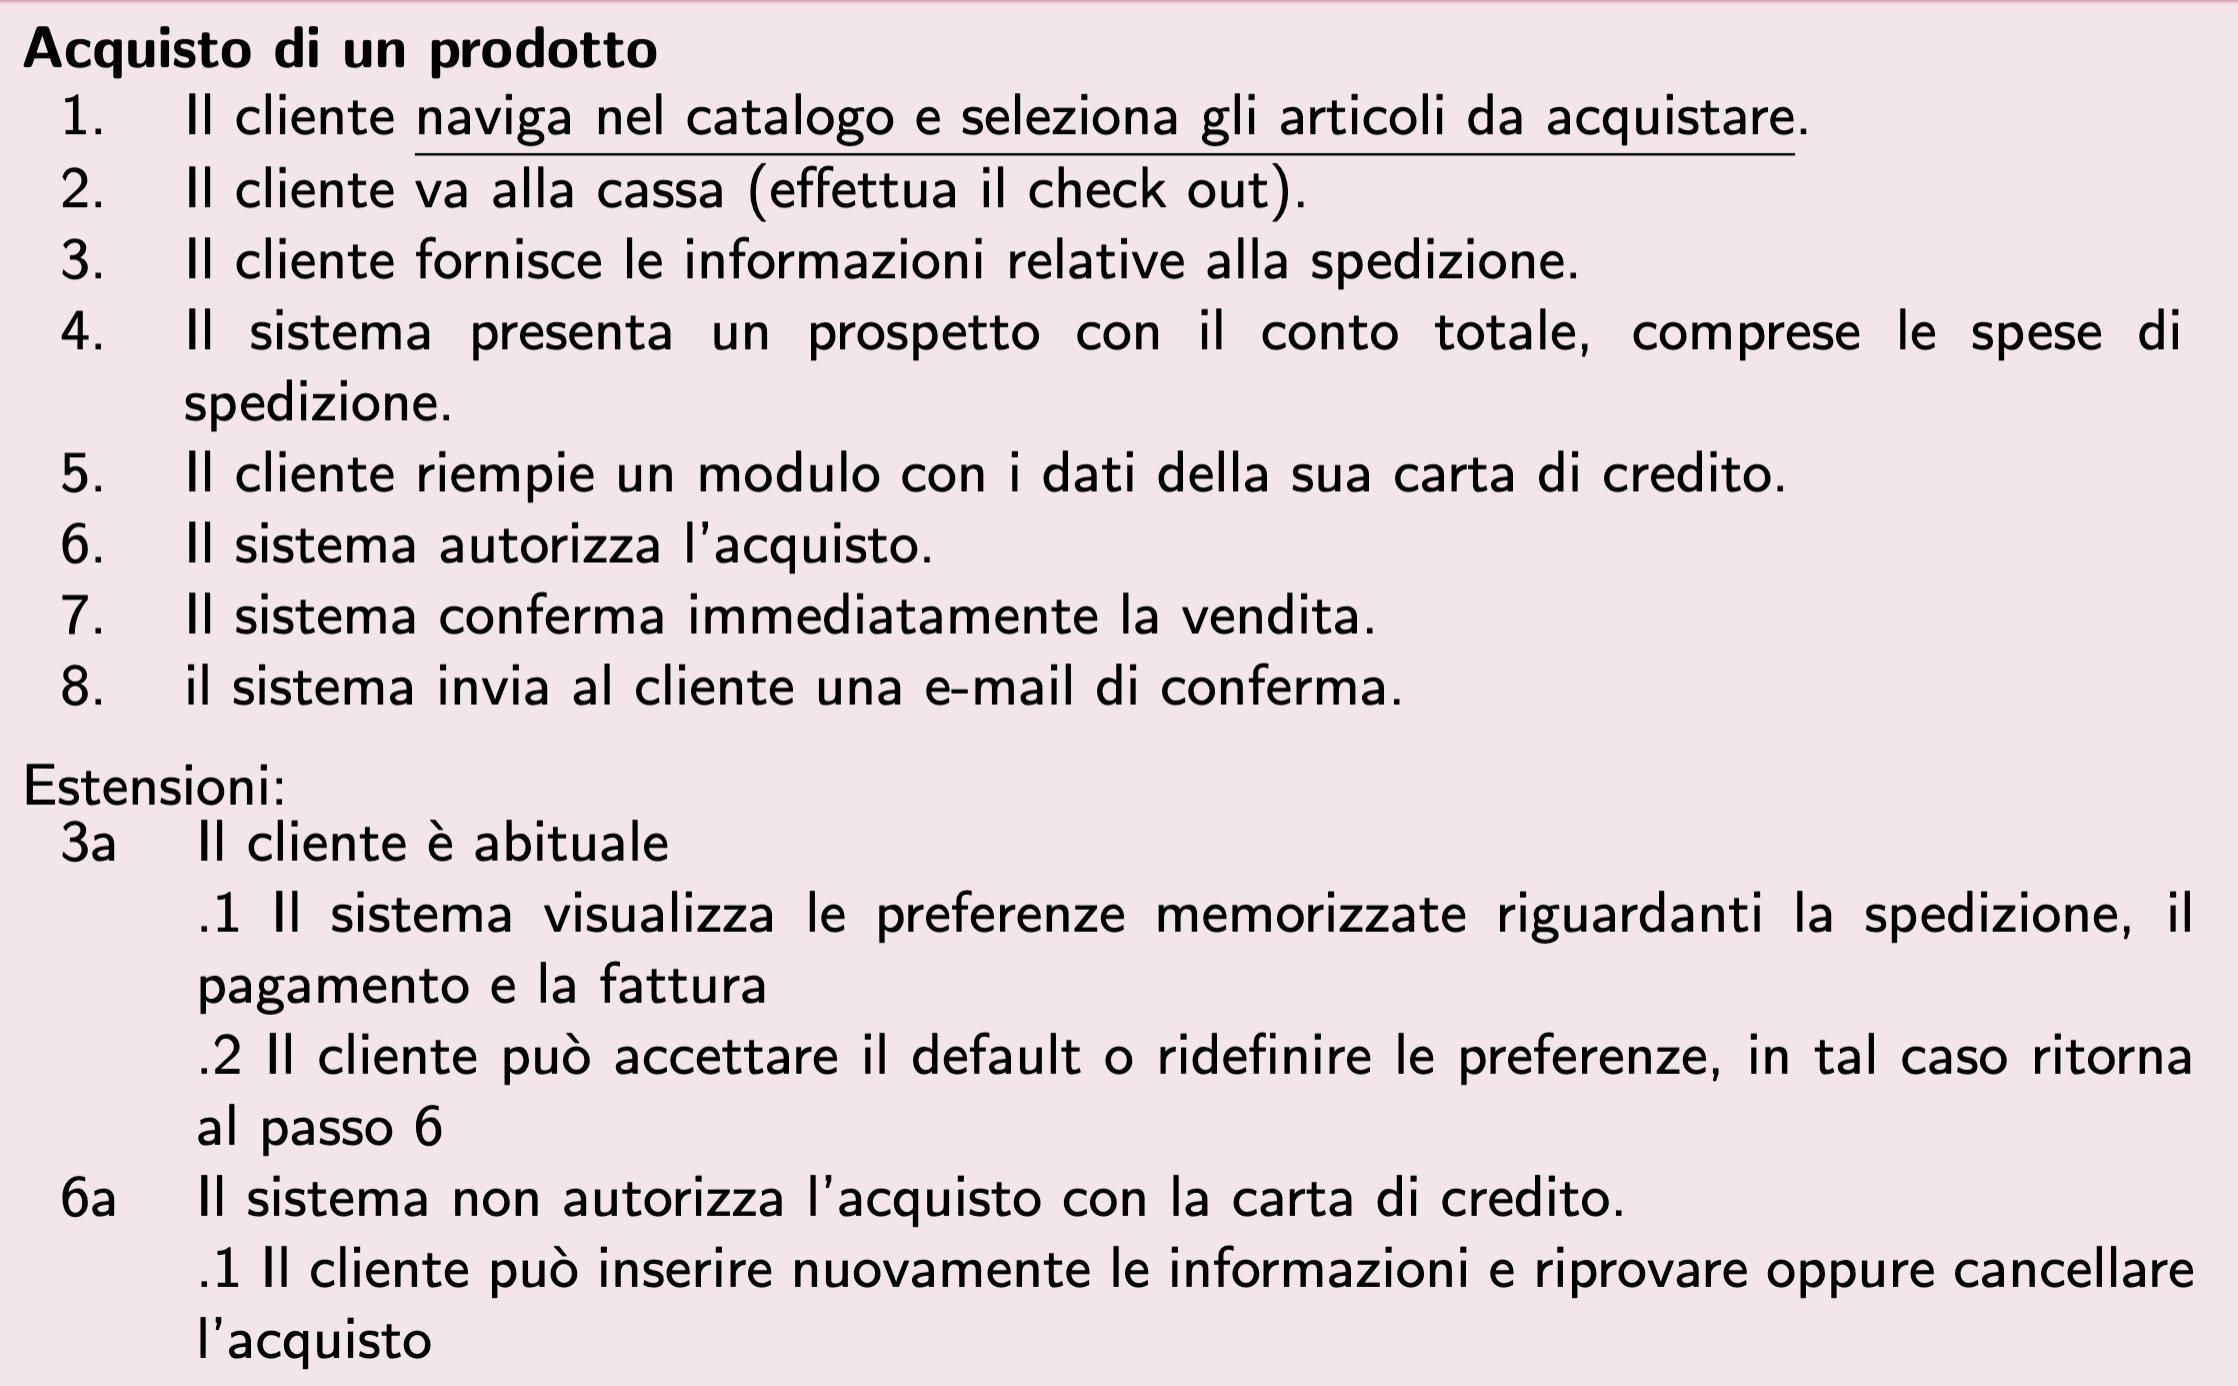
\includegraphics[width=0.48\linewidth]{assets/UML/use-case/use-case4.png}}
\end{figure}

\subparagraph{Inclusione} Scissione di un passo di un caso d'uso complicato, espresso come un altro caso d'uso completo (il primo \textit{include} il secondo). In forma testuale è sufficiente sottolineare il nome del caso d'uso incluso.

\textbf{\textit{Rappresentazione}}: linea tratteggiata che termina con una freccia (dipendenza) etichettata con la parola chiave $\langle\langle$include$\rangle\rangle$

\newpage

